\documentclass[10pt, aspectratio=169]{beamer}

% ═══════════════════════════════════════════════════════════════════════════
%  Professional Academic Theme — IIT Delhi branding
% ═══════════════════════════════════════════════════════════════════════════

% ── Theme ───────────────────────────────────────────────────────────────────
\usetheme{Madrid}
\useinnertheme{rectangles}
\beamertemplatenavigationsymbolsempty

% ── Colour Palette ─────────────────────────────────────────────────────────
\definecolor{iitdNavy}{HTML}{003B5C}
\definecolor{iitdDark}{HTML}{002642}
\definecolor{iitdAccent}{HTML}{0077B6}
\definecolor{iitdGray}{HTML}{4A5568}
\definecolor{iitdLightGray}{HTML}{E2E8F0}
\definecolor{alertRed}{HTML}{B91C1C}
\definecolor{successGreen}{HTML}{047857}

% ── Apply colours ──────────────────────────────────────────────────────────
\setbeamercolor{palette primary}{bg=iitdNavy, fg=white}
\setbeamercolor{palette secondary}{bg=iitdDark, fg=white}
\setbeamercolor{palette tertiary}{bg=iitdDark, fg=white}
\setbeamercolor{palette quaternary}{bg=iitdNavy, fg=white}
\setbeamercolor{structure}{fg=iitdNavy}
\setbeamercolor{frametitle}{bg=iitdNavy, fg=white}
\setbeamercolor{title}{fg=white, bg=iitdNavy}
\setbeamercolor{subtitle}{fg=iitdLightGray}
\setbeamercolor{author}{fg=white}
\setbeamercolor{institute}{fg=iitdLightGray}
\setbeamercolor{date}{fg=iitdLightGray}
\setbeamercolor{normal text}{fg=iitdGray}
\setbeamercolor{alerted text}{fg=alertRed}
\setbeamercolor{example text}{fg=successGreen}
\setbeamercolor{block title}{bg=iitdNavy, fg=white}
\setbeamercolor{block body}{bg=iitdLightGray!40, fg=iitdGray}
\setbeamercolor{block title alerted}{bg=alertRed!85!black, fg=white}
\setbeamercolor{block body alerted}{bg=alertRed!8, fg=iitdGray}
\setbeamercolor{block title example}{bg=successGreen!85!black, fg=white}
\setbeamercolor{block body example}{bg=successGreen!8, fg=iitdGray}
\setbeamercolor{itemize item}{fg=iitdNavy}
\setbeamercolor{itemize subitem}{fg=iitdAccent}
\setbeamercolor{enumerate item}{fg=iitdNavy}

% ── Fonts ──────────────────────────────────────────────────────────────────
\setbeamerfont{title}{size=\Large, series=\bfseries}
\setbeamerfont{frametitle}{size=\large, series=\bfseries}
\setbeamerfont{block title}{size=\normalsize, series=\bfseries}

% ── Bullets ────────────────────────────────────────────────────────────────
\setbeamertemplate{itemize item}{\small$\bullet$}
\setbeamertemplate{itemize subitem}{\scriptsize$\circ$}

% ── Footer ─────────────────────────────────────────────────────────────────
\setbeamertemplate{footline}{%
  \hfill%
  \usebeamercolor[fg]{normal text}%
  \usebeamerfont{footline}%
  \footnotesize\insertframenumber\,/\,\inserttotalframenumber%
  \hspace{8pt}\vspace{4pt}%
}

% ── Packages ───────────────────────────────────────────────────────────────
\usepackage{graphicx}
\usepackage{booktabs}
\usepackage[table]{xcolor}
\usepackage{amsmath,amssymb}
\usepackage{siunitx}
\usepackage{tikz}
\usetikzlibrary{positioning}
\usepackage{hyperref}
\usepackage{multicol}
\usepackage{caption}
\captionsetup{font=small, labelformat=empty}

\graphicspath{{../doe/cross_campaign/figures/}{../doe/surrogate/figures/}{../doe/results_full/cases/case_03/figures/}}

% ── Key Insight box ────────────────────────────────────────────────────────
\newcommand{\keyinsight}[1]{%
  \begin{beamercolorbox}[wd=\textwidth, sep=6pt, rounded=true]{block body}
    \textcolor{iitdNavy}{\textbf{\small$\star$\;Key Insight:}}\;
    {\small #1}
  \end{beamercolorbox}%
}

% ═══════════════════════════════════════════════════════════════════════════
\begin{document}

% ─── SLIDE 1: TITLE ──────────────────────────────────────────────────────────
\begin{frame}[plain]
    \begin{tikzpicture}[remember picture, overlay]
        \shade[left color=iitdDark, right color=iitdAccent!80!iitdNavy,
               shading angle=15]
            (current page.south west) rectangle (current page.north east);
        \fill[white, opacity=0.06]
            ([xshift=-2cm, yshift=-2.5cm]current page.north east) circle (6cm);
        \fill[white, opacity=0.04]
            ([xshift=2.5cm, yshift=2cm]current page.south west) circle (4.5cm);
        \draw[iitdAccent!60!white, line width=0.8pt]
            ([xshift=2cm, yshift=-0.5cm]current page.west)
            -- ([xshift=-2cm, yshift=-0.5cm]current page.east);

        \node[anchor=south, text width=0.85\paperwidth, align=center]
            at ([yshift=1.0cm]current page.center) {
                {\LARGE\bfseries\color{white}%
                 Multiobjective Optimization of Hydrogen\\[6pt]
                 Injection into Natural Gas Pipelines}\\[14pt]
                {\large\color{iitdLightGray}A Surrogate-Assisted Approach}\\[14pt]
                {\large\color{iitdAccent!80!white}\textbf{CLD880 - Minor Project Presentation}}
            };

        \node[anchor=north, text width=0.75\paperwidth, align=center]
            at ([yshift=-1.2cm]current page.center) {
                {\large\color{white}\textbf{Sakhare Yash Balram}\;\;{\normalsize (2022CH71496)}}\\[8pt]
                {\large\color{iitdLightGray}%
                 Supervisor: \textbf{Prof.\ Abhijeet Raj}}\\[6pt]
                {\normalsize\color{iitdLightGray}%
                 Department of Chemical Engineering\\
                 Indian Institute of Technology Delhi}\\[10pt]
                {\small\color{iitdLightGray!80}May 2026}
            };
    \end{tikzpicture}
\end{frame}

% ═══════════════════════════════════════════════════════════════════════════
\section{Motivation}
% ═══════════════════════════════════════════════════════════════════════════

% ─── SLIDE 2: THE REAL PROBLEM ────────────────────────────────────────────
\begin{frame}{The Problem: H\texorpdfstring{$_2$}{2} Blending into Gas Grids}
    \begin{columns}[T]
        \begin{column}{0.55\textwidth}
            \textbf{Hydrogen-Natural Gas Blending (HBNG)} is the cheapest
            path to decarbonise the gas grid without rebuilding it.

            \vspace{0.6em}
            \textbf{The density mismatch drives stratification:}
            \begin{itemize}
                \item H$_2$ is \textbf{8$\times$ lighter} than CH$_4$
                      ($0.082$ vs $0.668$~kg/m$^3$).
                \item Buoyancy pushes H$_2$ to the pipe crown instead
                      of mixing uniformly.
            \end{itemize}

            \vspace{0.6em}
            \begin{table}
                \centering\scriptsize
                \begin{tabular}{@{}lccc@{}}
                    \toprule
                    \textbf{Property} & \textbf{CH$_4$} & \textbf{H$_2$} & \textbf{Ratio} \\
                    \midrule
                    Density (kg/m$^3$) & 0.668 & 0.082 & $8\times$ \\
                    Vol.\ energy (MJ/m$^3$) & 36 & 11 & $3\times$ \\
                    Flammability (\%vol) & 5-15 & 4-76 & $5\times$ wider \\
                    \bottomrule
                \end{tabular}
            \end{table}
        \end{column}
        \begin{column}{0.42\textwidth}
            \begin{alertblock}{Downstream Consequences}
                \small
                \begin{itemize}
                    \item \textbf{Hydrogen embrittlement} at the pipe
                          crown (localised high $p_{\text{H}_2}$).
                    \item \textbf{Wobbe Index drift} $\to$ combustion
                          instability at end-burners.
                    \item \textbf{Metering errors} from
                          composition-dependent speed of sound.
                \end{itemize}
            \end{alertblock}

            \vspace{0.3em}
            {\small Uniform mixing is a safety and regulatory
            requirement, not just an optimisation goal.}
        \end{column}
    \end{columns}
\end{frame}

% ─── SLIDE 3: CONTRIBUTION ───────────────────────────────────────────────
\begin{frame}{Our Contribution - Closing the Gap}
    \begin{columns}[T]
        \begin{column}{0.50\textwidth}
            \alert{\textbf{Gap:} No study treats injection angle
            $\alpha$ as a primary design variable, and none performs
            bi-objective (CoV, $\Delta P$) optimisation.}

            \vspace{0.6em}
            \textbf{This project:}
            \begin{enumerate}
                \item Sweep $(\alpha, d/D, \text{VR})$ on equal footing.
                \item Top vs.\ bottom injection (buoyancy control).
                \item 4 campaigns, 40 validated CFD cases.
                \item GPR surrogate + NSGA-II Pareto search.
            \end{enumerate}
        \end{column}
        \begin{column}{0.47\textwidth}
            \vspace{0.5em}
            \textbf{Design Variables:}
            \begin{table}
                \centering\scriptsize
                \begin{tabular}{@{}lll@{}}
                    \toprule
                    \textbf{Variable} & \textbf{Symbol} & \textbf{Range} \\
                    \midrule
                    Injection angle & $\alpha$ & $30^\circ$, $90^\circ$ \\
                    Diameter ratio & $d/D$ & 0.15-0.45 \\
                    Velocity ratio & VR & 0.69-5.84 \\
                    Injection side & - & Top / Bottom \\
                    \bottomrule
                \end{tabular}
            \end{table}

            \vspace{0.5em}
            \textbf{Formal MOO:}
            \[
                \min_{\mathbf{x}} \;
                \mathbf{F}(\mathbf{x}) = \begin{bmatrix}
                    \text{CoV}(\mathbf{x}) \\[4pt]
                    |\Delta P|(\mathbf{x})
                \end{bmatrix}
            \]

            \vspace{0.3em}
            {\small First simultaneous optimisation of mixing
            quality and pumping cost for T-junction H$_2$ injection.}
        \end{column}
    \end{columns}
\end{frame}

% ═══════════════════════════════════════════════════════════════════════════
\section{Methodology}
% ═══════════════════════════════════════════════════════════════════════════

% ─── SLIDE 4: METHODOLOGY OVERVIEW ───────────────────────────────────────
\begin{frame}[fragile]{Methodology Overview}
    \small
    \begin{columns}[T]
        \begin{column}{0.52\textwidth}
            \textbf{Solver \& Physics:}
            \begin{itemize}\setlength{\itemsep}{0pt}
                \item OpenFOAM \texttt{rhoReactingBuoyantFoam}
                \item $k$-$\omega$~SST, compressible, buoyancy-coupled
                \item Half-domain symmetry ($x \ge 0$)
            \end{itemize}

            \vspace{0.2em}
            \textbf{Operating Conditions:}
            \begin{itemize}\setlength{\itemsep}{0pt}
                \item Main: $D = 0.46$~m, $u = 10$~m/s,
                      CH$_4$, $P = 6.9$~MPa
                \item Branch: H$_2$,
                      $u_{\text{br}} = \text{VR} \cdot u_{\text{main}}$
            \end{itemize}

            \vspace{0.2em}
            \textbf{Metrics:}
            \begin{itemize}\setlength{\itemsep}{0pt}
                \item \textbf{CoV} = $\sigma(Y_{\text{H}_2}) / \bar{Y}_{\text{H}_2}$ at outlet
                \item \textbf{$|\Delta P|$} = LP-filtered pressure drop
                      on $[0.4, 1.2]$~s
            \end{itemize}
        \end{column}
        \begin{column}{0.45\textwidth}
            \textbf{Design of Experiments:}
            \begin{itemize}\setlength{\itemsep}{0pt}
                \item Sliced LHS: 5~$d/D$ bins $\times$ 2~VR per bin
                      = 10 cases/campaign
                \item Same seed $\to$ matched-pair control
                \item 4 campaigns: $\{30^\circ, 90^\circ\} \times
                      \{\text{top, bottom}\}$
            \end{itemize}

            \vspace{0.3em}
            \begin{center}
                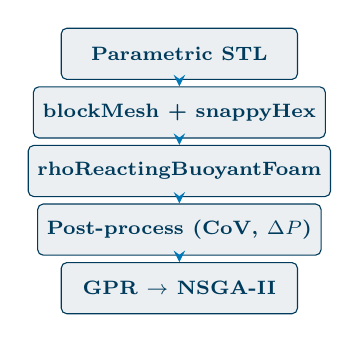
\begin{tikzpicture}[
                    wfbox/.style={draw=iitdNavy, fill=iitdNavy!8,
                                  rounded corners=2pt, minimum height=0.65cm,
                                  minimum width=3.0cm, align=center,
                                  font=\scriptsize\bfseries, text=iitdNavy},
                    arr/.style={->, >=stealth, thick, color=iitdAccent},
                    node distance=0.08cm
                ]
                    \node[wfbox] (s1) {Parametric STL};
                    \node[wfbox, below=of s1] (s2) {blockMesh + snappyHex};
                    \node[wfbox, below=of s2] (s3) {rhoReactingBuoyantFoam};
                    \node[wfbox, below=of s3] (s4) {Post-process (CoV, $\Delta P$)};
                    \node[wfbox, below=of s4] (s5) {GPR $\to$ NSGA-II};
                    \draw[arr] (s1) -- (s2);
                    \draw[arr] (s2) -- (s3);
                    \draw[arr] (s3) -- (s4);
                    \draw[arr] (s4) -- (s5);
                \end{tikzpicture}
            \end{center}
        \end{column}
    \end{columns}
\end{frame}

% ─── SLIDE 5: MESH & VALIDATION ─────────────────────────────────────────
\begin{frame}{Mesh and Validation}
    \begin{columns}[T]
        \begin{column}{0.50\textwidth}
            \begin{figure}
                \centering
                
\includegraphics[width=0.92\linewidth]{fig_mesh_xz.png}
                \caption{Mesh on the $x=0$ symmetry plane ($90^\circ$, case~03).
                Boundary layers visible at walls.}
            \end{figure}
        \end{column}
        \begin{column}{0.48\textwidth}
            \textbf{Mesh statistics (typical):}
            \begin{table}
                \centering\scriptsize
                \begin{tabular}{@{}lr@{}}
                    \toprule
                    Half-domain cells & $\sim$463\,k \\
                    Max non-orthogonality & $49^\circ$ \\
                    Layer coverage & 99.6\% \\
                    $y^+$ & $\sim$1 \\
                    \bottomrule
                \end{tabular}
            \end{table}

            \vspace{0.3em}
            \textbf{Grid independence (3 levels):}
            \begin{table}
                \centering\scriptsize
                \begin{tabular}{@{}lcc@{}}
                    \toprule
                    \textbf{Mesh} & $\Delta$CoV & $\Delta|\Delta P|$ \\
                    \midrule
                    230k $\to$ 460k & 0.4\% & 1.6\% \\
                    460k $\to$ 920k & 0.2\% & 0.7\% \\
                    \bottomrule
                \end{tabular}
            \end{table}

            \vspace{0.3em}
            \textbf{All 40 cases pass:}
            \begin{itemize}\small
                \item Cumulative continuity error $<10^{-2}$
                \item Residuals $<10^{-8}$
                \item Mass balance $<0.5\%$
                \item No NaN / FPE
            \end{itemize}
        \end{column}
    \end{columns}
\end{frame}

% ─── SLIDE 6: RESULTS WALKTHROUGH (TOP) ────────────────────────────────
\begin{frame}{Results Walkthrough: Case~04 ($90^\circ$ Top, VR = 3.81, CoV = 0.066)}
    \centering\vspace{-0.3em}
    \begin{columns}[T]
        \begin{column}{0.33\textwidth}
            \centering
            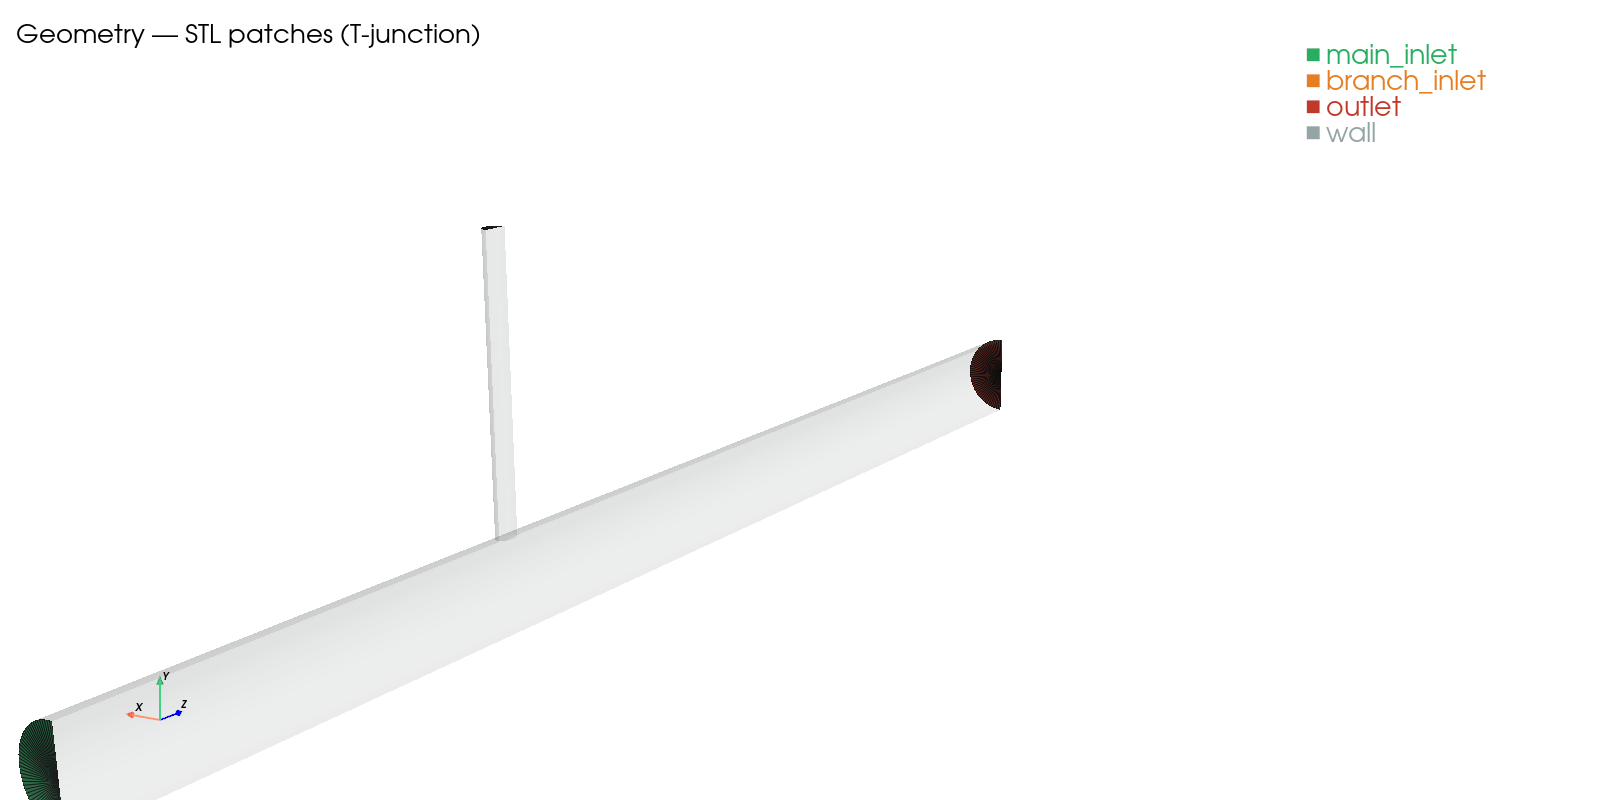
\includegraphics[width=0.95\linewidth]{../doe/results_full/cases/case_04/figures/fig_geometry.png}\\[-0.4em]
            {\scriptsize\textbf{(a)} T-junction geometry}
        \end{column}
        \begin{column}{0.33\textwidth}
            \centering
            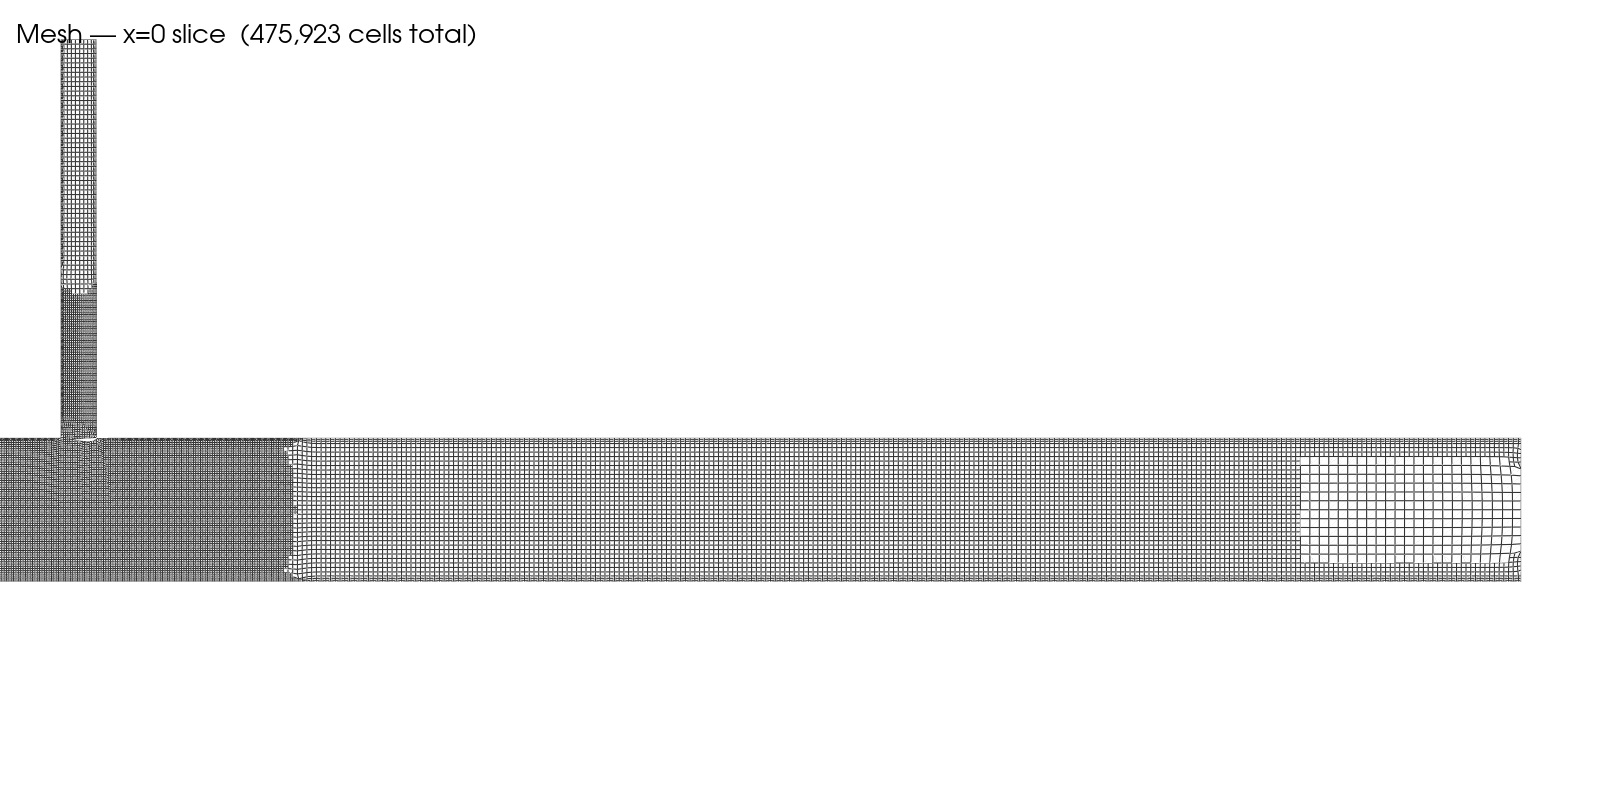
\includegraphics[width=0.95\linewidth]{../doe/results_full/cases/case_04/figures/fig_mesh_xz.png}\\[-0.4em]
            {\scriptsize\textbf{(b)} Mesh on $x\!=\!0$ plane (476k cells)}
        \end{column}
        \begin{column}{0.33\textwidth}
            \centering
            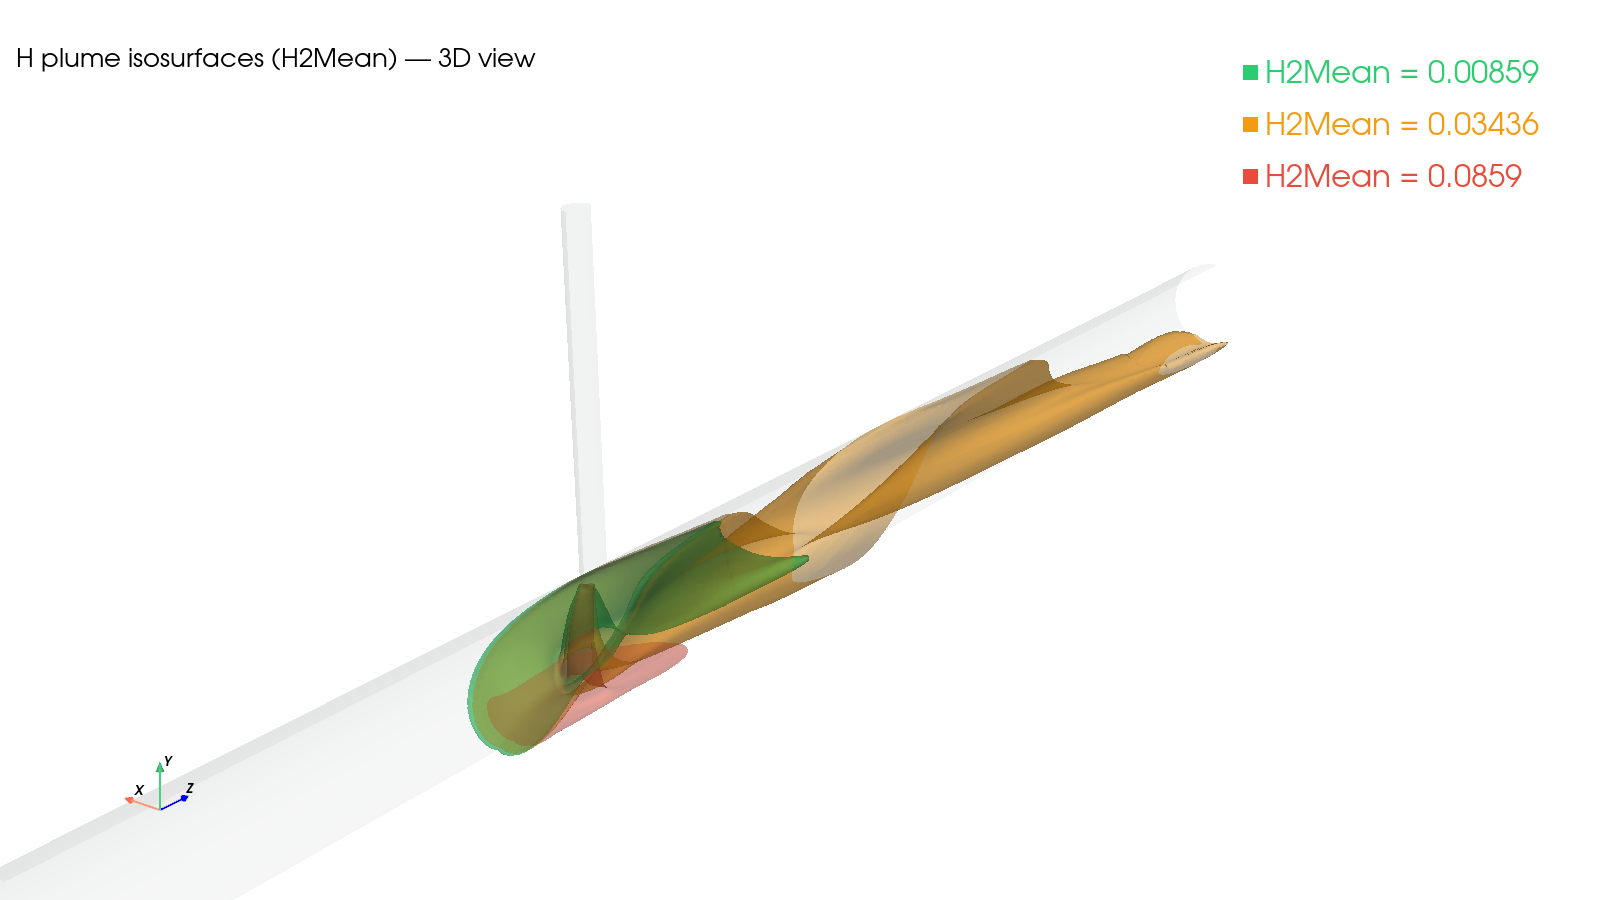
\includegraphics[width=0.95\linewidth]{../doe/results_full/cases/case_04/figures/fig_H2_isosurface.png}\\[-0.4em]
            {\scriptsize\textbf{(c)} H$_2$ isosurfaces (3D plume)}
        \end{column}
    \end{columns}

    \vspace{0.25em}
    \begin{columns}[T]
        \begin{column}{0.33\textwidth}
            \centering
            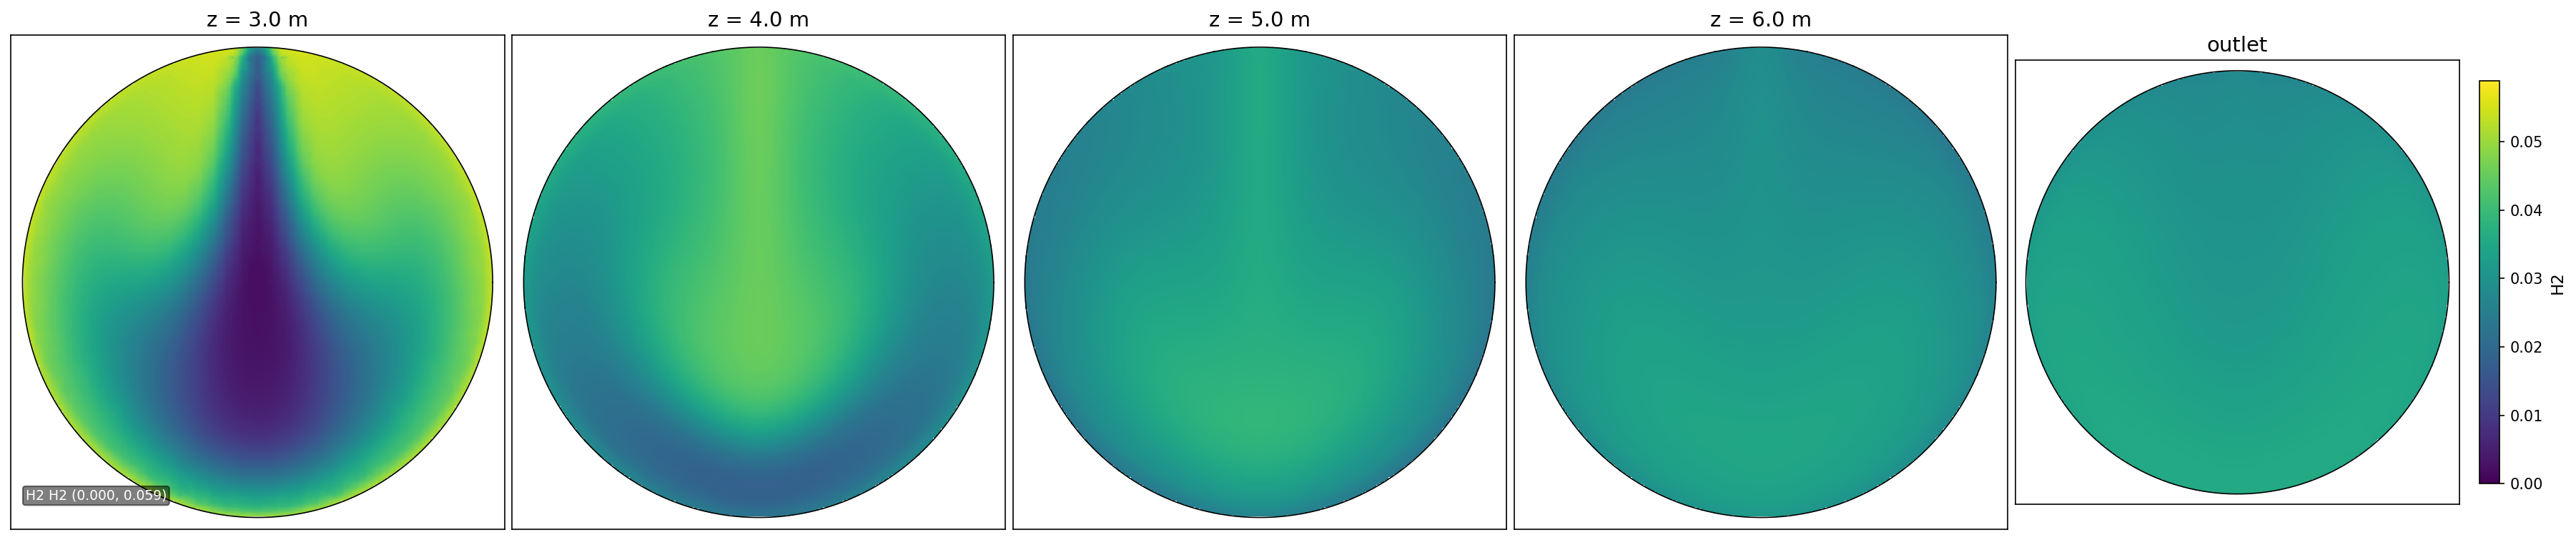
\includegraphics[width=0.95\linewidth]{../doe/results_full/cases/case_04/figures/fig_H2_strip.png}\\[-0.4em]
            {\scriptsize\textbf{(d)} H$_2$ at $z\!=\!3,4,5,6$\,m + outlet}
        \end{column}
        \begin{column}{0.33\textwidth}
            \centering
            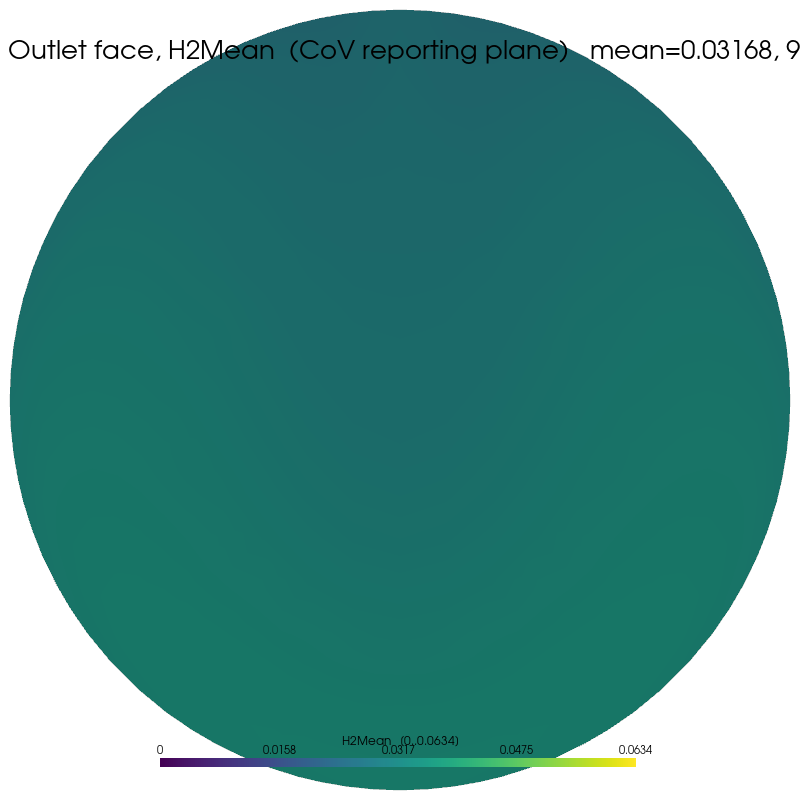
\includegraphics[width=0.65\linewidth]{../doe/results_full/cases/case_04/figures/fig_H2_outlet.png}\\[-0.4em]
            {\scriptsize\textbf{(e)} Outlet: nearly uniform}
        \end{column}
        \begin{column}{0.33\textwidth}
            \centering
            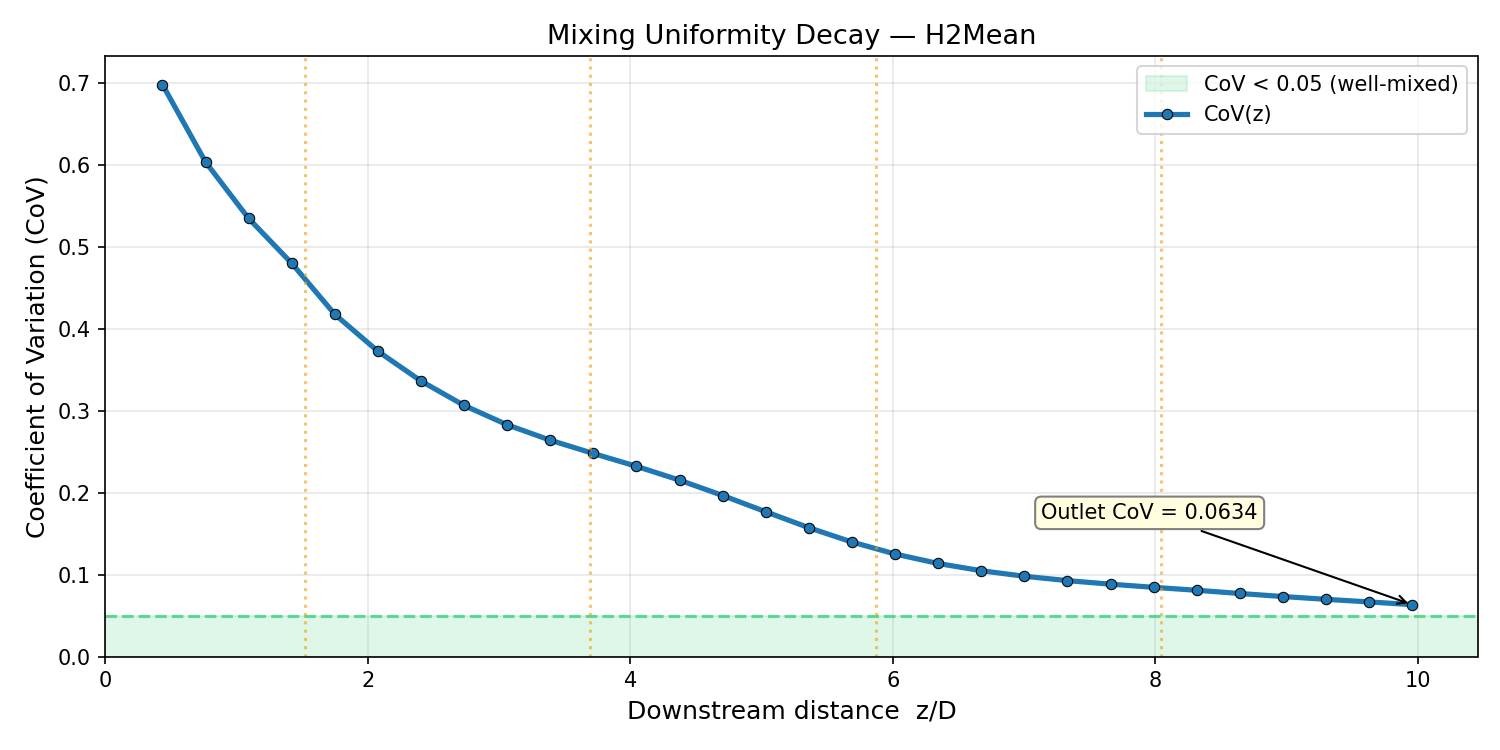
\includegraphics[width=0.95\linewidth]{../doe/results_full/cases/case_04/figures/fig_CoV_vs_zD.png}\\[-0.4em]
            {\scriptsize\textbf{(f)} CoV: 0.70 $\to$ 0.063}
        \end{column}
    \end{columns}
\end{frame}

% ─── SLIDE 7: SAME CASE — BOTTOM INJECTION ────────────────────────────
\begin{frame}{Same Case, Bottom Injection: CoV = 0.066 $\to$ 0.271 ($4\times$ worse)}
    \centering\vspace{-0.3em}
    {\footnotesize Same $90^\circ$, $d/D = 0.252$, VR = 3.81 - only injection side changed.}

    \vspace{0.15em}
    \begin{columns}[T]
        \begin{column}{0.33\textwidth}
            \centering
            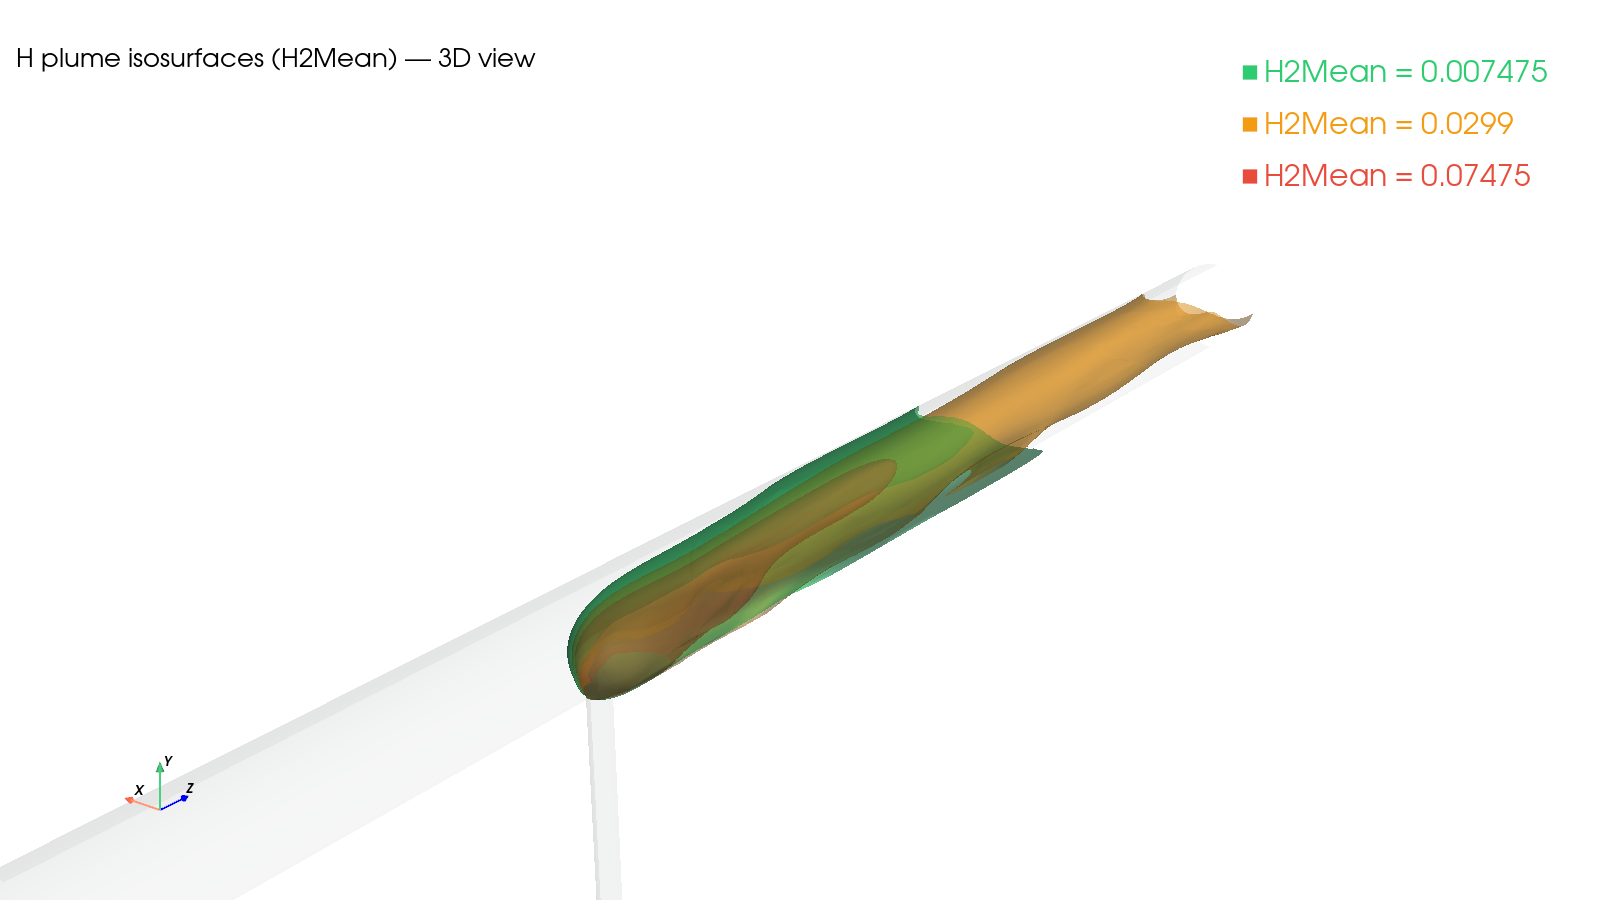
\includegraphics[width=0.95\linewidth]{../doe/results_full_90deg_bottom/case_04/figures/fig_H2_isosurface.png}\\[-0.4em]
            {\scriptsize\textbf{(a)} H$_2$ plume rises as narrow column}
        \end{column}
        \begin{column}{0.33\textwidth}
            \centering
            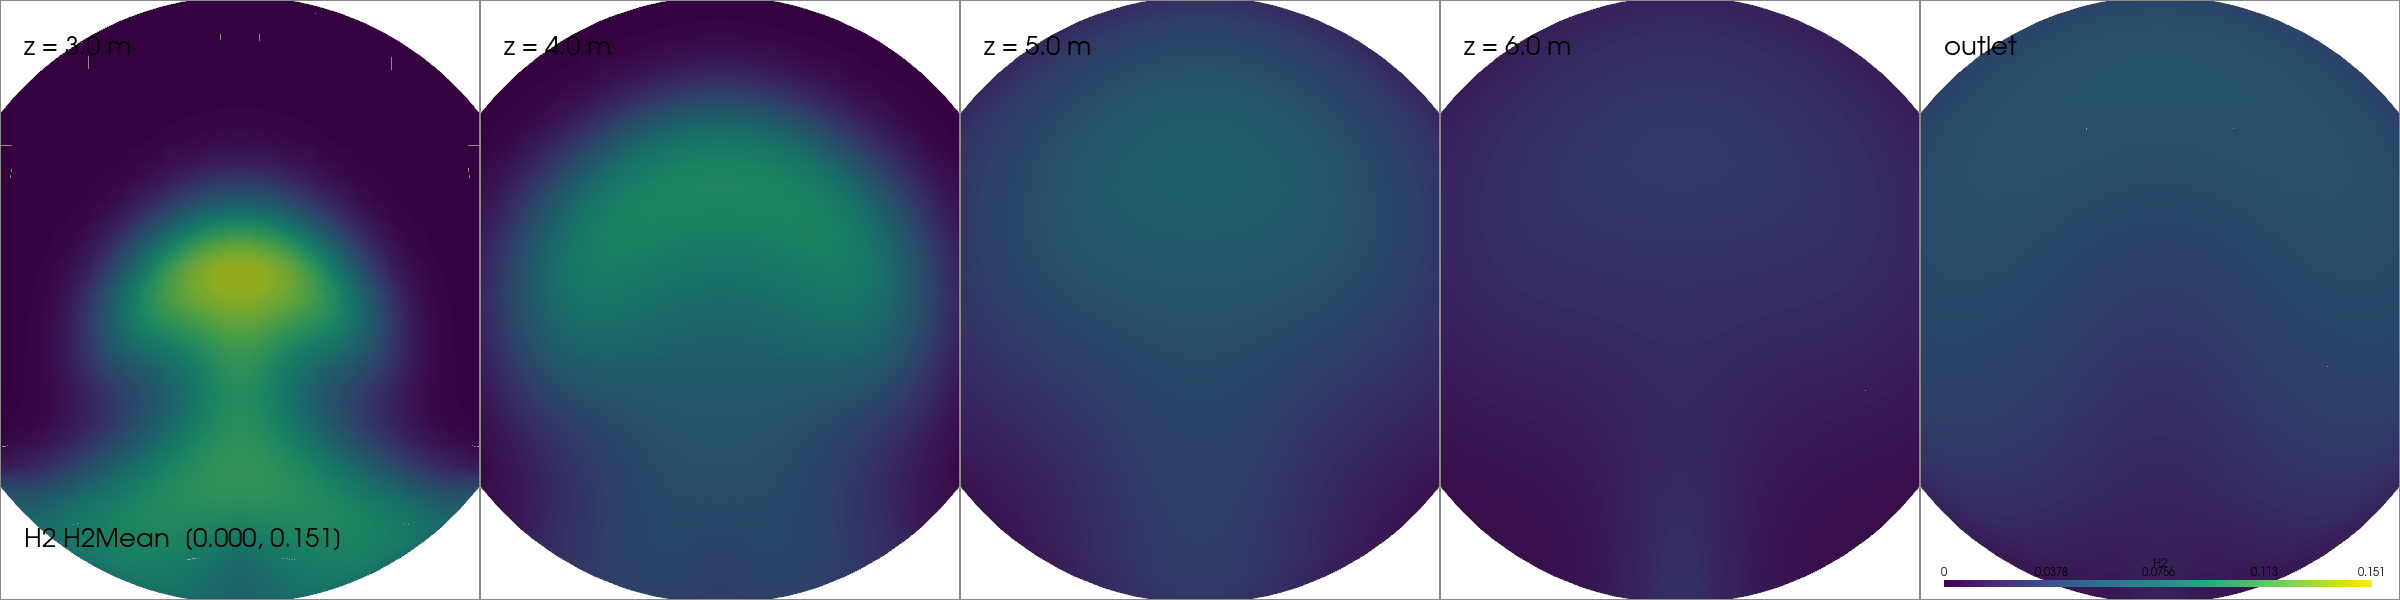
\includegraphics[width=0.95\linewidth]{../doe/results_full_90deg_bottom/case_04/figures/fig_H2_strip.png}\\[-0.4em]
            {\scriptsize\textbf{(b)} Crown streak persists to outlet}
        \end{column}
        \begin{column}{0.33\textwidth}
            \centering
            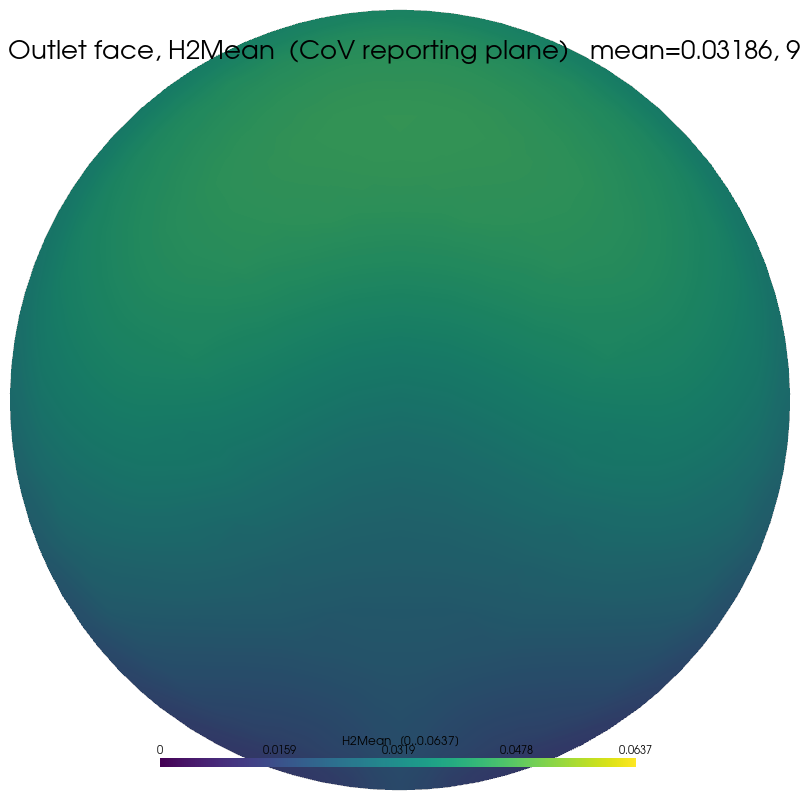
\includegraphics[width=0.65\linewidth]{../doe/results_full_90deg_bottom/case_04/figures/fig_H2_outlet.png}\\[-0.4em]
            {\scriptsize\textbf{(c)} Outlet: strong gradient remains}
        \end{column}
    \end{columns}

    \vspace{0.2em}
    \begin{columns}[T]
        \begin{column}{0.50\textwidth}
            \centering
            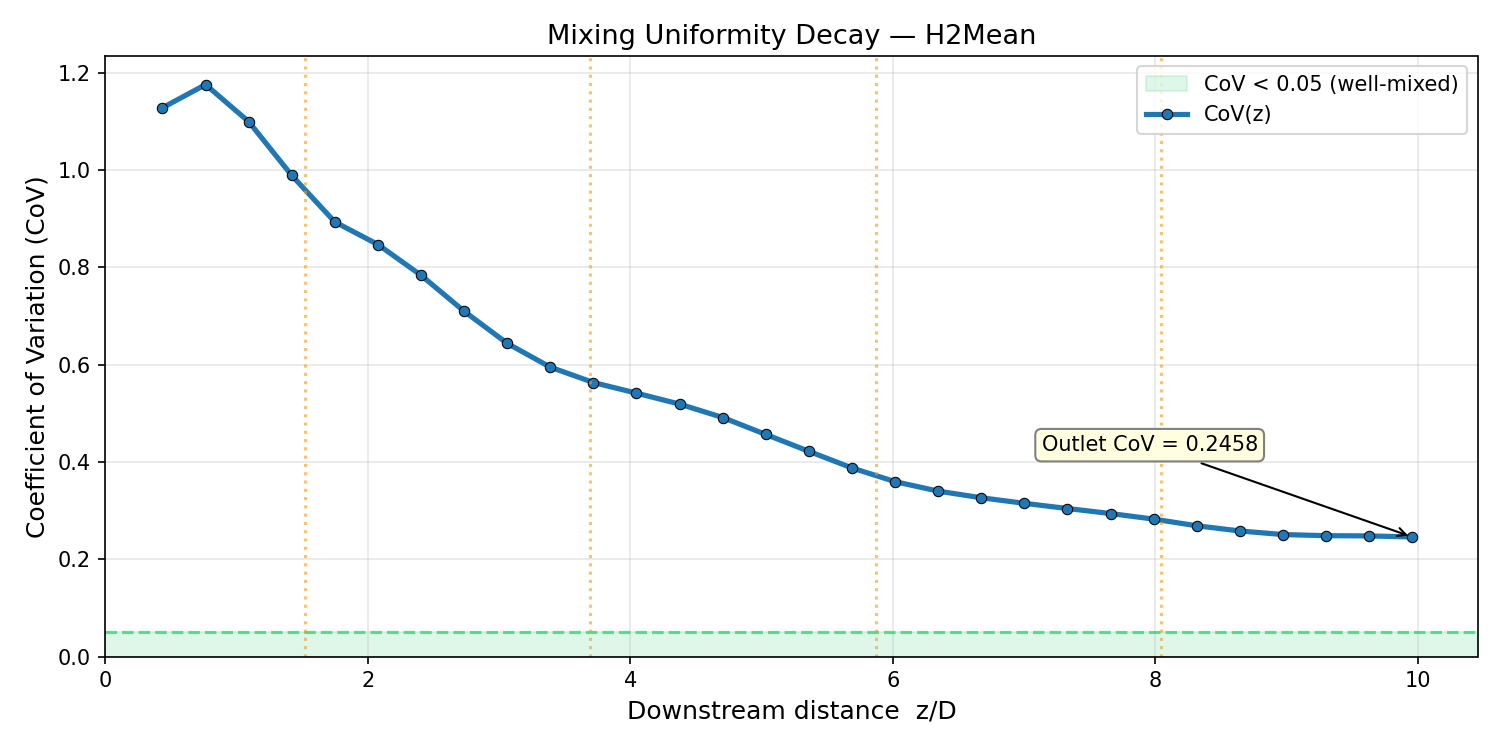
\includegraphics[width=0.85\linewidth]{../doe/results_full_90deg_bottom/case_04/figures/fig_CoV_vs_zD.png}\\[-0.4em]
            {\scriptsize\textbf{(d)} CoV $\to$ 0.246 - never reaches 0.05 target}
        \end{column}
        \begin{column}{0.50\textwidth}
            \vspace{1em}
            {\small All 17 matched pairs: top injection wins
            every time ($p = 1.5 \times 10^{-5}$).
            Median degradation: $+109\%$ at $90^\circ$,
            $+324\%$ at $30^\circ$. $|\Delta P|$ is unchanged.}
        \end{column}
    \end{columns}
\end{frame}

% ═══════════════════════════════════════════════════════════════════════════
\section{Results}
% ═══════════════════════════════════════════════════════════════════════════

% ─── SLIDE 7: VR EFFECT (same angle, same d/D) ─────────────────────────
\begin{frame}{Velocity Ratio Effect: Same Geometry, Different VR}
    \centering
    {\footnotesize $90^\circ$ top, $d/D = 0.252$ - only VR differs.
    Cross-sections at $z = 3, 4, 5, 6$\,m and outlet.}

    \vspace{0.1em}
    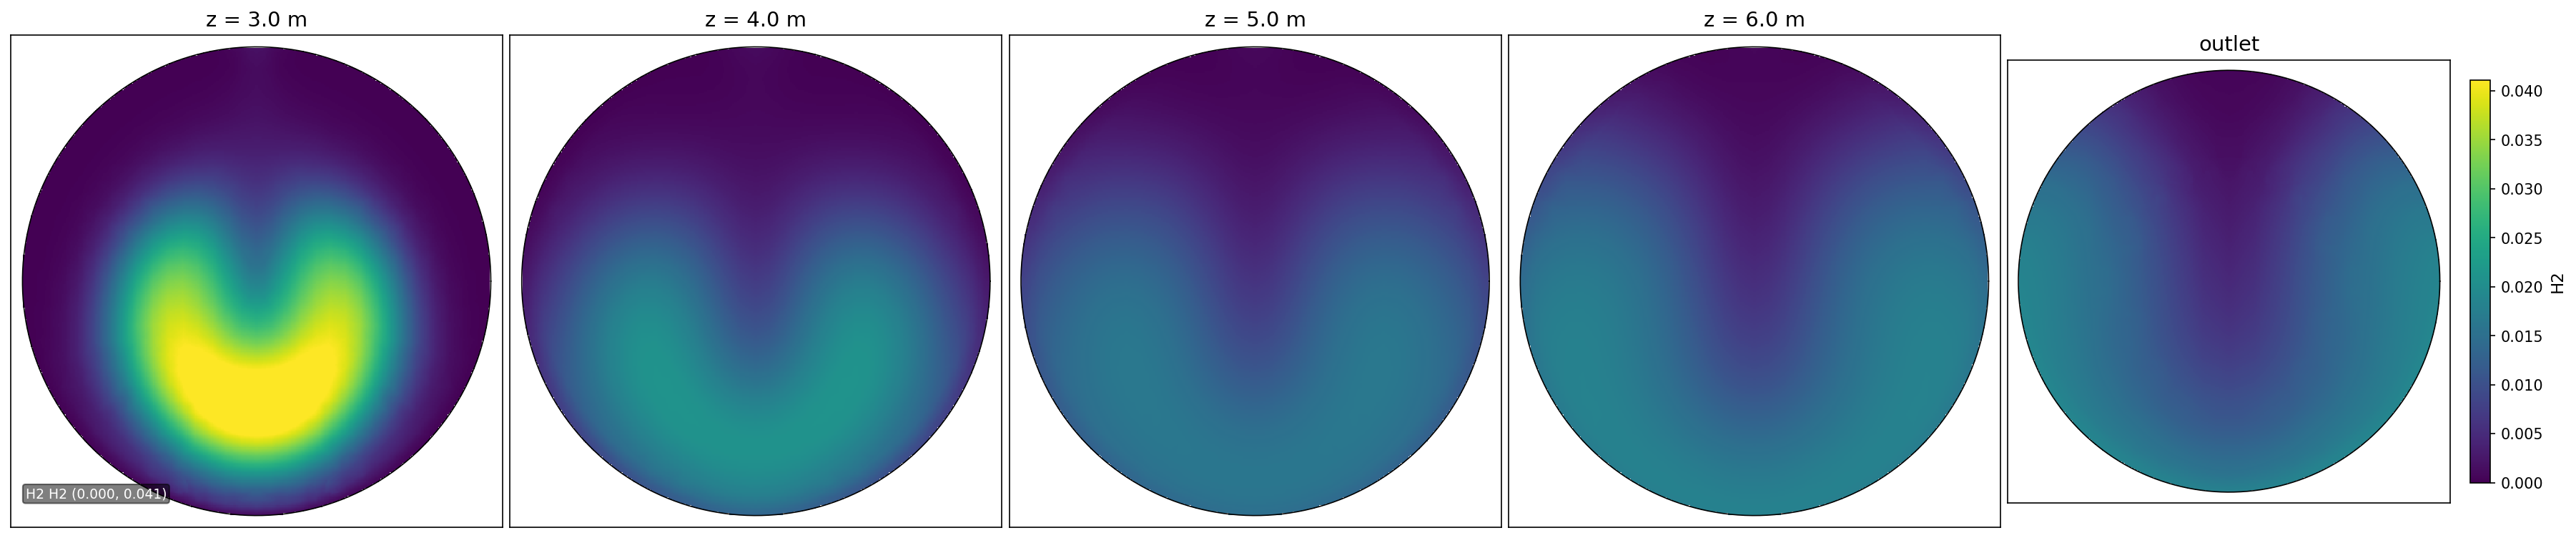
\includegraphics[width=0.74\linewidth,trim=0 5 0 30,clip]{../doe/results_full/cases/case_03/figures/fig_H2_strip.png}\\[-0.5em]
    {\scriptsize Case~03: \textbf{VR = 1.33}, CoV = \textbf{0.472} --
    H$_2$ hugs the crown; dark bottom = unmixed CH$_4$.}

    \vspace{0.05em}
    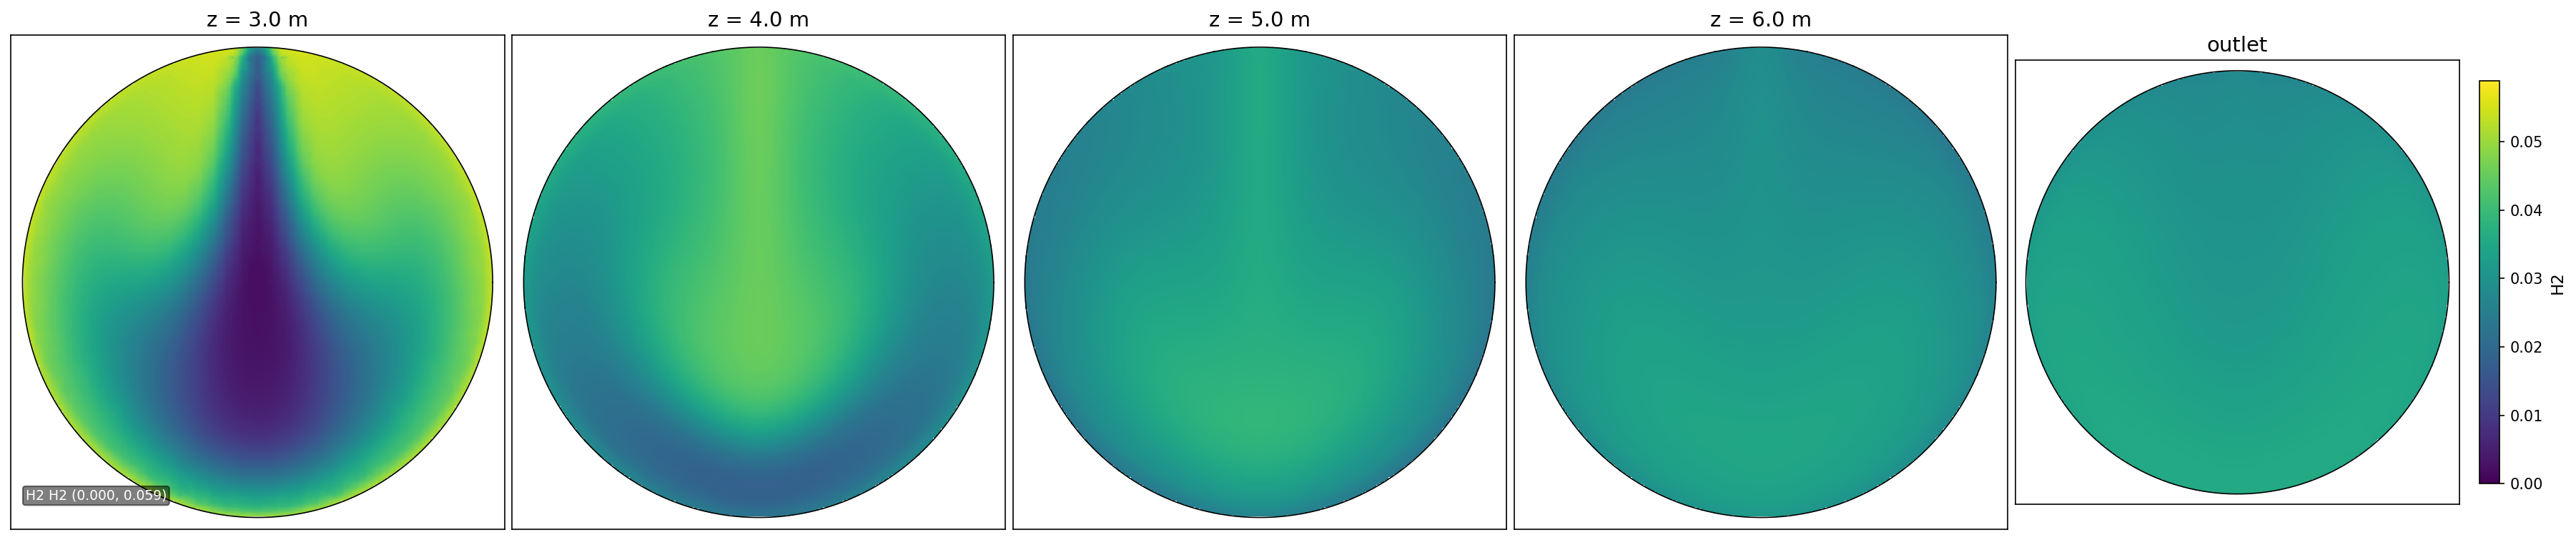
\includegraphics[width=0.74\linewidth,trim=0 5 0 30,clip]{../doe/results_full/cases/case_04/figures/fig_H2_strip.png}\\[-0.5em]
    {\scriptsize Case~04: \textbf{VR = 3.81}, CoV = \textbf{0.066} --
    Jet penetrates past centreline; uniform by $z = 5$\,m.}

    \vspace{0.1em}
    {\small Same pipe, same branch.
    Tripling VR ($1.33 \to 3.81$) cuts CoV by $7\times$.
    VR is the strongest lever on mixing.}
\end{frame}

% ─── SLIDE 7: ANGLE EFFECT (same design point, different angle) ─────────
\begin{frame}{Angle Effect: Same Design Point, $90^\circ$ vs $30^\circ$}
    \centering
    {\footnotesize $d/D = 0.296$, VR = 2.61, HBR = 0.187 - only angle differs.
    Cross-sections at $z = 3, 4, 5, 6$\,m and outlet.}

    \vspace{0.1em}
    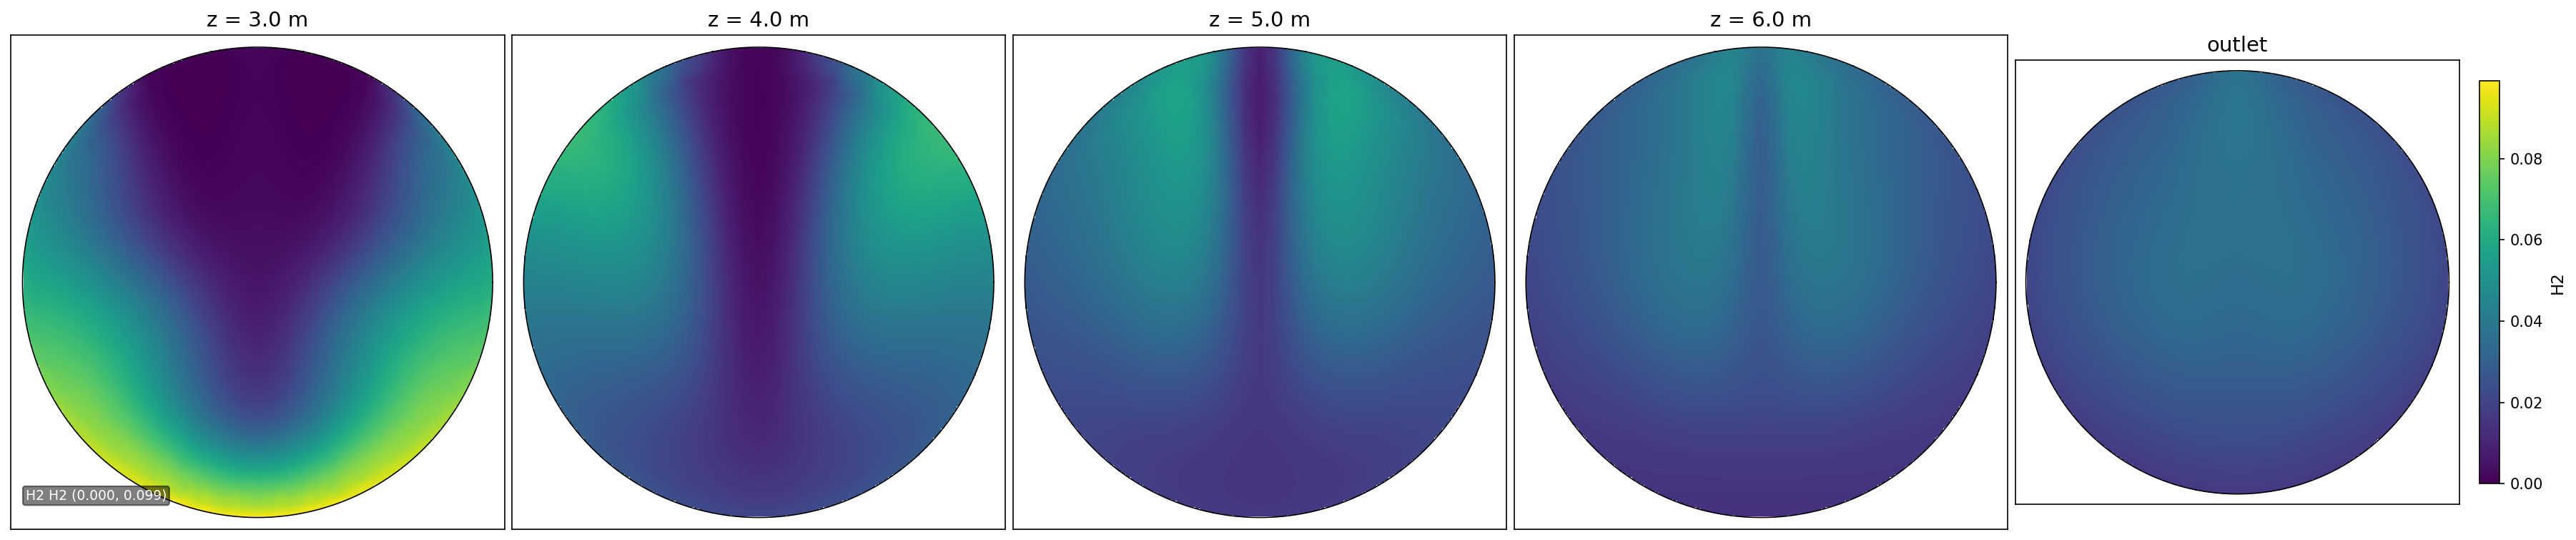
\includegraphics[width=0.74\linewidth,trim=0 5 0 30,clip]{../doe/results_full/cases/case_06/figures/fig_H2_strip.png}\\[-0.5em]
    {\scriptsize $\mathbf{90^\circ}$, case~06: CoV = \textbf{0.202} --
    Vertical streaks persist to outlet; crown-bottom asymmetry remains.}

    \vspace{0.05em}
    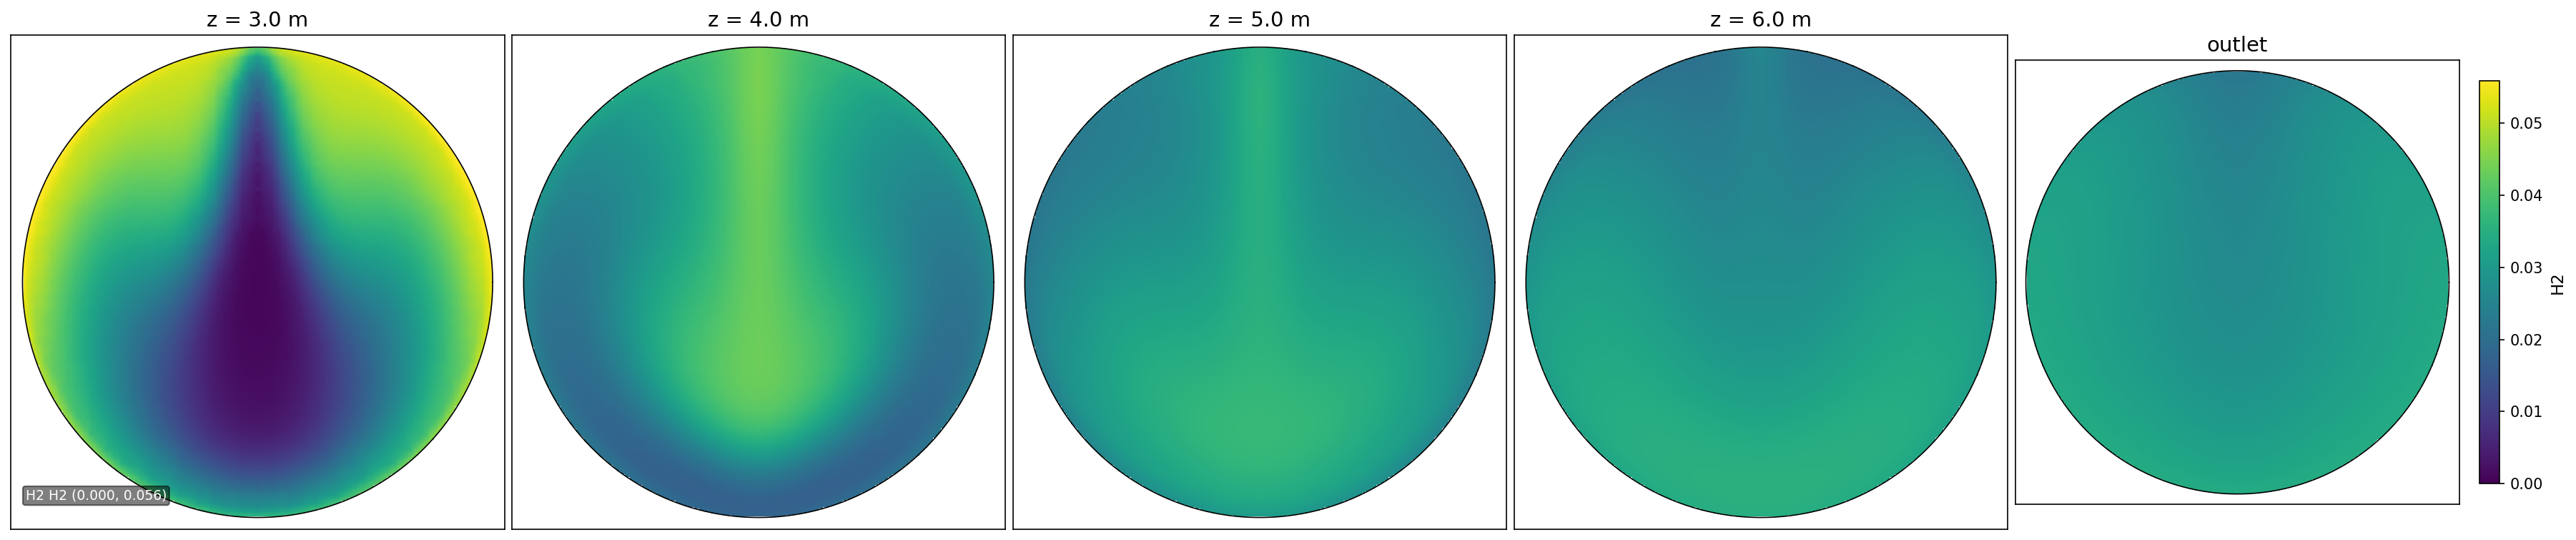
\includegraphics[width=0.74\linewidth,trim=0 5 0 30,clip]{../doe/results_full_30deg/cases/case_06/figures/fig_H2_strip.png}\\[-0.5em]
    {\scriptsize $\mathbf{30^\circ}$, case~06: CoV = \textbf{0.088} --
    Teardrop plume at $z=3$\,m homogenises by $z=5$\,m; outlet is uniform.}

    \vspace{0.1em}
    {\small Identical design point, only angle changed.
    All 7 matched pairs: median CoV drops $46\%$, $|\Delta P|$ drops $63\%$ ($p = 0.008$).}
\end{frame}

% ─── SLIDE 10: POWER-LAW SCALING ────────────────────────────────────────
\begin{frame}{Power-Law Scaling: CoV vs VR}
    \begin{columns}[T]
        \begin{column}{0.52\textwidth}
            \begin{figure}
                \centering
                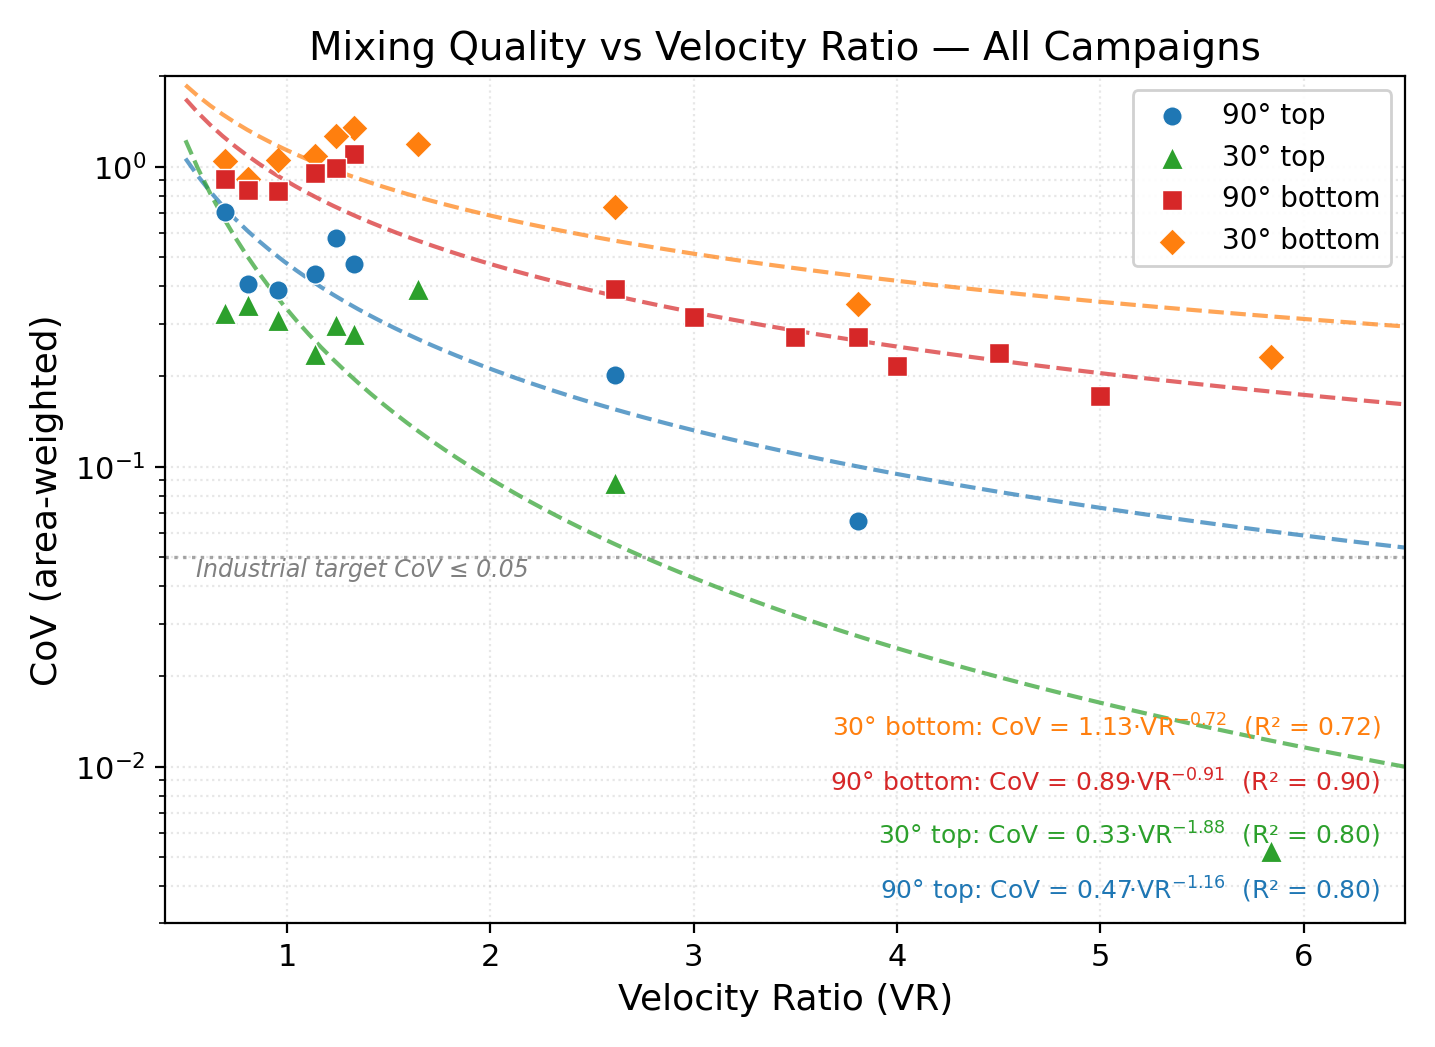
\includegraphics[width=\linewidth]{fig1_CoV_vs_VR.png}
                \caption{Log-log fit of CoV vs VR for all four campaigns.
                Dashed line: CoV = 0.05 target.}
            \end{figure}
        \end{column}
        \begin{column}{0.46\textwidth}
            \begin{table}
                \centering\scriptsize
                \begin{tabular}{@{}lcc@{}}
                    \toprule
                    \textbf{Campaign} & \textbf{Fit} & $R^2$ \\
                    \midrule
                    $90^\circ$ top & $0.47\,\text{VR}^{-1.16}$ & 0.80 \\
                    \rowcolor{successGreen!12}
                    $\mathbf{30^\circ}$ \textbf{top} & $\mathbf{0.33\,\text{VR}^{-1.88}}$ & \textbf{0.80} \\
                    $90^\circ$ bot & $0.89\,\text{VR}^{-0.91}$ & 0.90 \\
                    $30^\circ$ bot & $1.13\,\text{VR}^{-0.72}$ & 0.72 \\
                    \bottomrule
                \end{tabular}
            \end{table}

            \vspace{0.5em}
            The exponent for $30^\circ$~top ($b = -1.88$) is
            \textbf{$1.6\times$} steeper than for $90^\circ$~top
            ($b = -1.16$).

            \vspace{0.4em}
            Each unit of VR buys \textbf{nearly twice as much mixing
            improvement} on the tilted geometry.

            \vspace{0.4em}
            Bottom-injection exponents are shallower --
            buoyancy limits how much mixing VR can buy.
        \end{column}
    \end{columns}
\end{frame}

% ─── SLIDE 11: PARETO FRONTIER ──────────────────────────────────────────
\begin{frame}{Pareto Front: The Trade-Off Visualised}
    \begin{columns}[T]
        \begin{column}{0.52\textwidth}
            \centering
            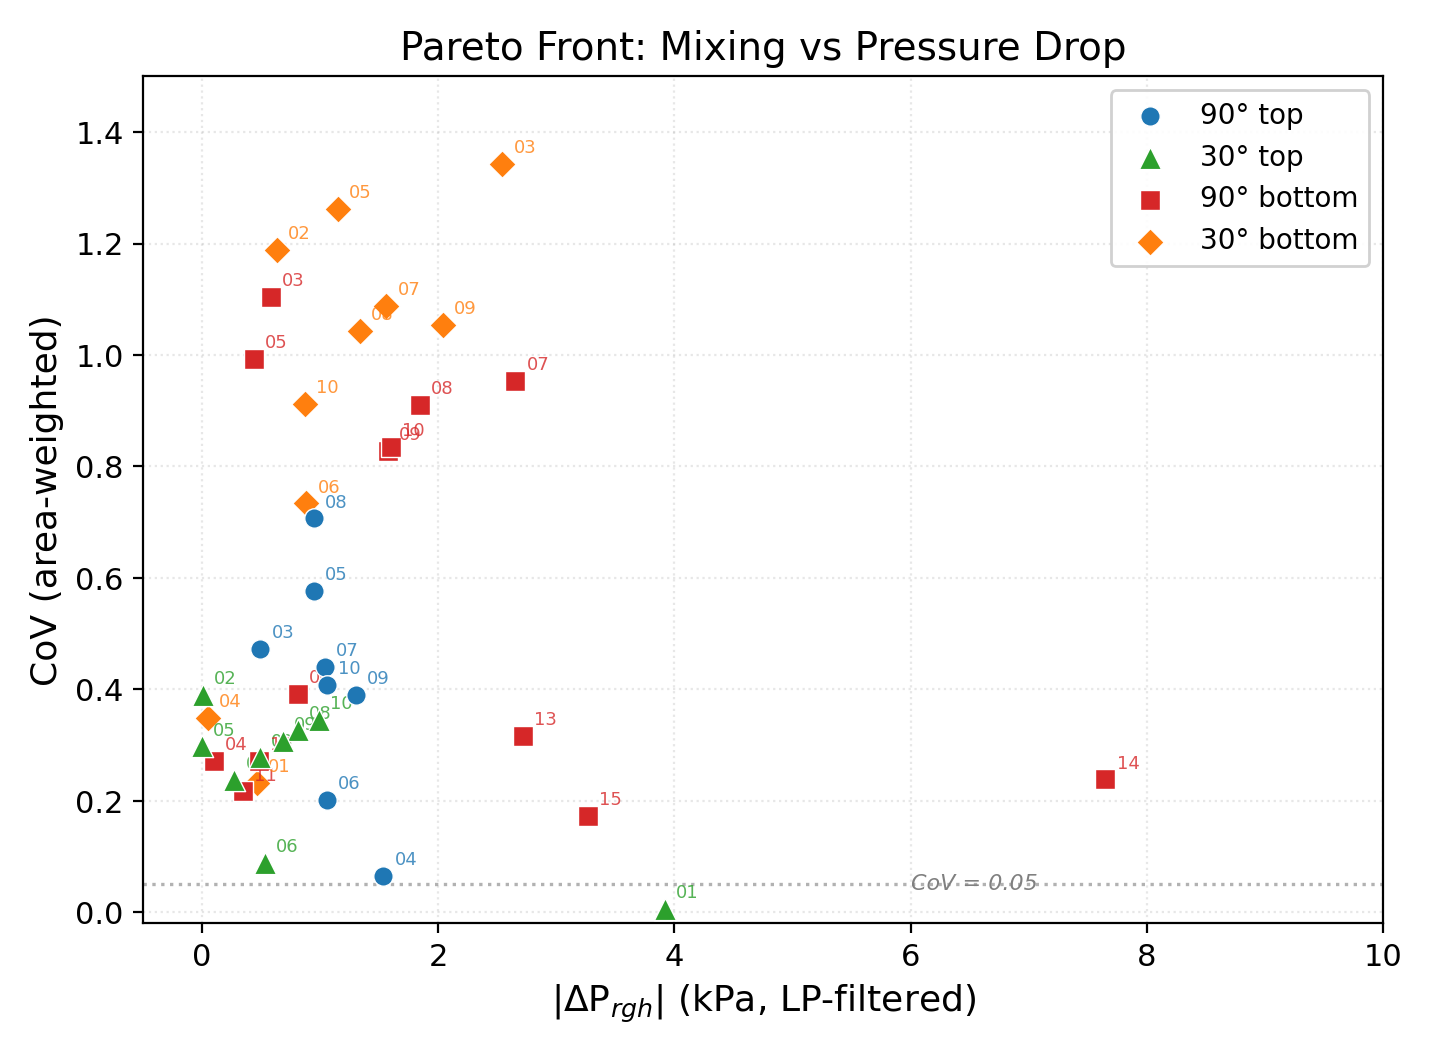
\includegraphics[width=\linewidth]{fig3_pareto.png}\\[-0.3em]
            {\scriptsize Four-campaign Pareto front. Lower-left is better
            (low CoV, low $|\Delta P|$).}
        \end{column}
        \begin{column}{0.45\textwidth}
            \textbf{$30^\circ$ top} occupies the desirable lower-left corner.

            \vspace{0.3em}
            \textbf{Standout cases:}
            \begin{itemize}\setlength{\itemsep}{0.1em}
                \item \textbf{Best mixing:} Case~01 ($30^\circ$ top) --
                      CoV = 0.005 at $|\Delta P| \approx 4.2$~kPa.
                \item \textbf{Cheapest:} Case~09 ($30^\circ$ top) --
                      $|\Delta P| \approx 0.3$~kPa with CoV = 0.31.
            \end{itemize}

            \vspace{0.2em}
            Every $90^\circ$ point is dominated by some $30^\circ$ point.
            No bottom-injection point reaches CoV $\le 0.05$.

            \vspace{0.3em}
            {\small $30^\circ$ top is the only configuration
            that consistently reaches CoV $< 0.05$.}
        \end{column}
    \end{columns}
\end{frame}

% ─── SLIDE 12: PHYSICAL MECHANISM ───────────────────────────────────────
\begin{frame}{Physical Mechanism: Why Does Tilt + Top Work?}
    \begin{columns}[T]
        \begin{column}{0.50\textwidth}
            \begin{figure}
                \centering
                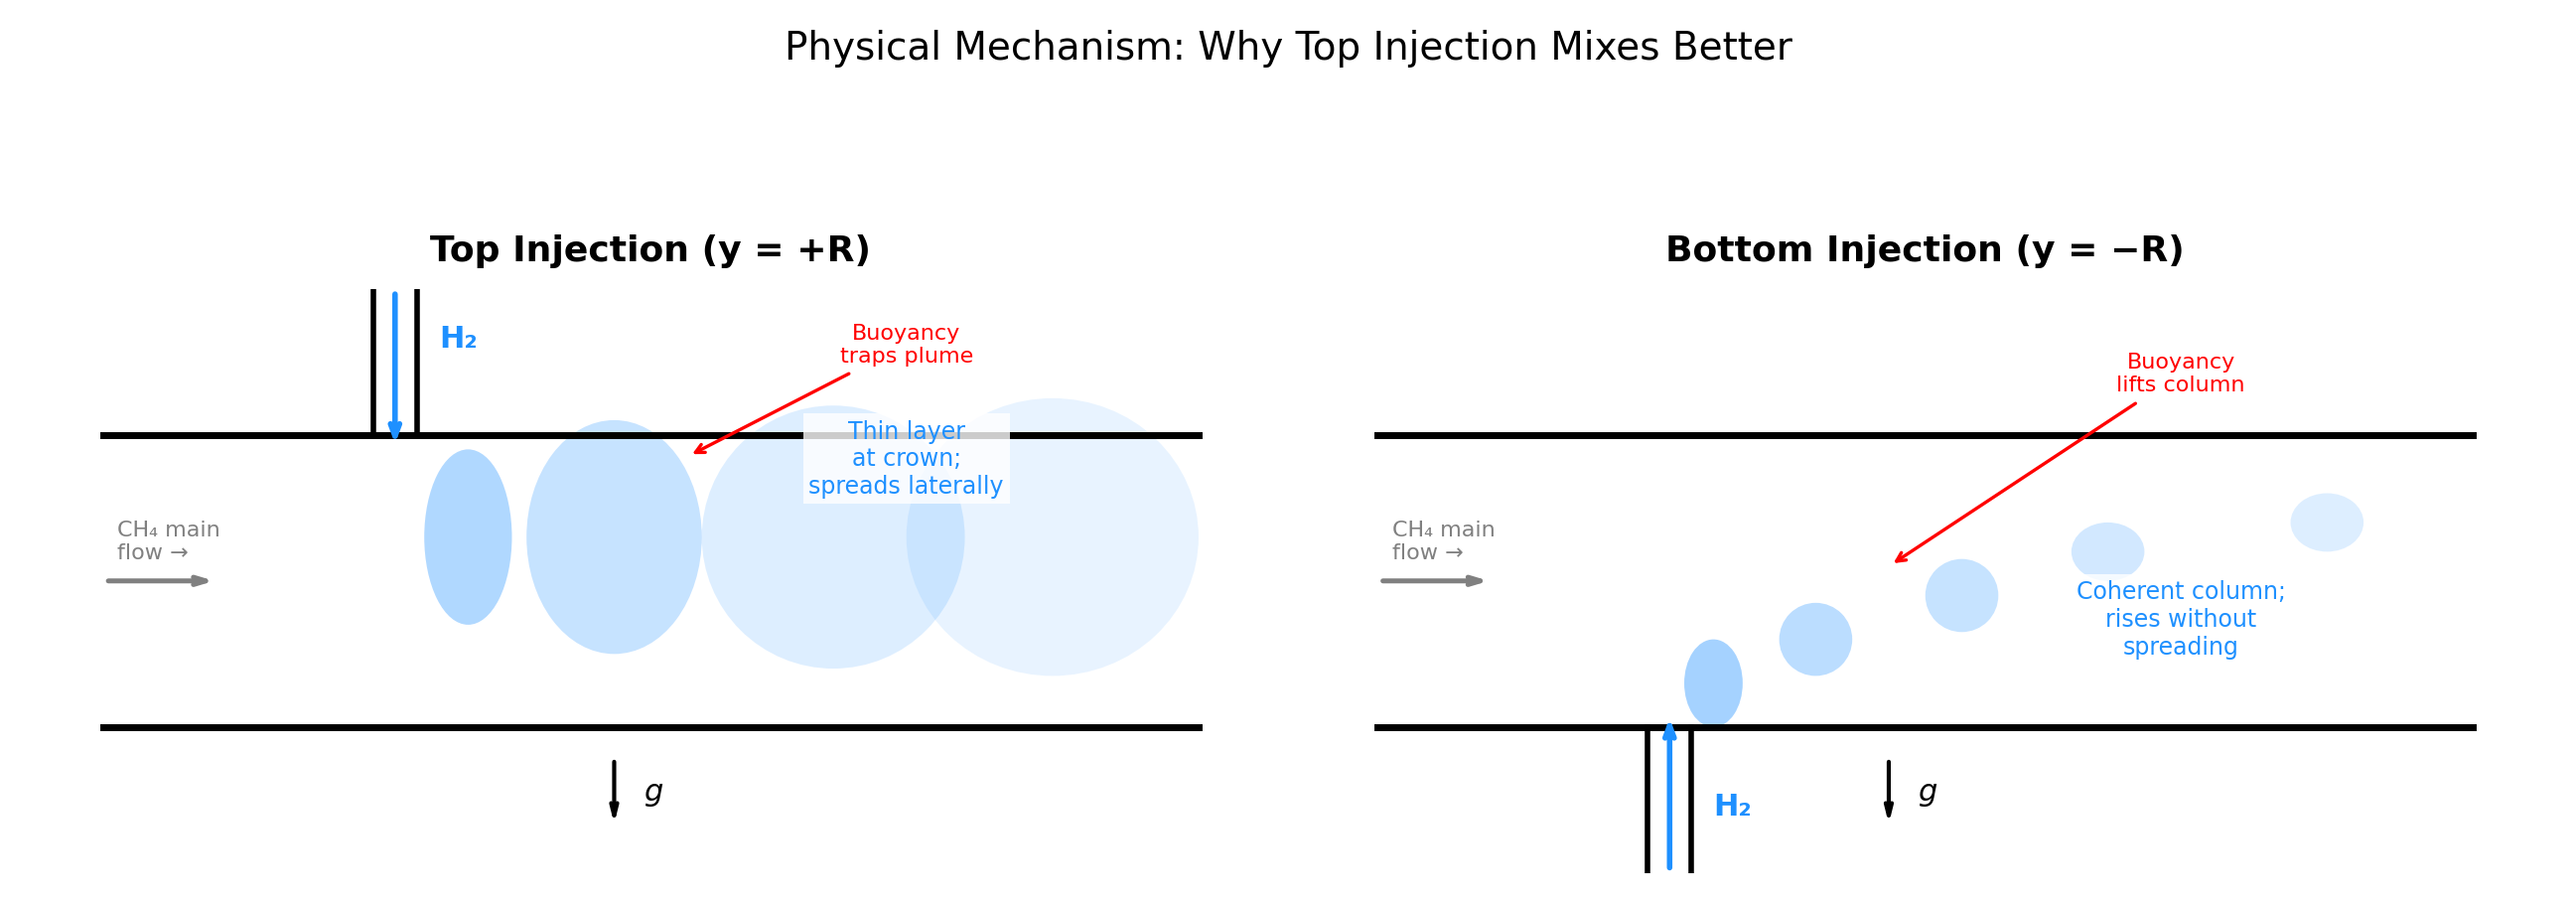
\includegraphics[width=\linewidth]{fig6_mechanism_schematic.png}
                \caption{Buoyancy mechanism. Left: top injection spreads
                H$_2$ laterally. Right: bottom injection lifts a
                coherent column.}
            \end{figure}
        \end{column}
        \begin{column}{0.47\textwidth}
            \small
            \textbf{Two synergistic effects:}

            \vspace{0.2em}
            \textbf{1.\ Tilt ($30^\circ$ vs $90^\circ$):}
            \begin{itemize}\setlength{\itemsep}{0pt}
                \item $90^\circ$ jet impinges on opposite wall,
                      traps a low-H$_2$ core.
                \item $30^\circ$ jet feeds a streamwise shear layer
                      entraining CH$_4$ along the pipe.
                \item Momentum aligned with flow $\to$ lower $|\Delta P|$.
            \end{itemize}

            \vspace{0.2em}
            \textbf{2.\ Buoyancy (top vs bottom):}
            \begin{itemize}\setlength{\itemsep}{0pt}
                \item Top: buoyancy \emph{opposes} jet $\to$
                      thin wide layer, large diffusion area.
                \item Bottom: buoyancy \emph{assists} jet $\to$
                      narrow column, small diffusion area.
            \end{itemize}

        \end{column}
    \end{columns}
\end{frame}

% ═══════════════════════════════════════════════════════════════════════════
\section{Surrogate Modelling}
% ═══════════════════════════════════════════════════════════════════════════

% ─── SLIDE 13: SURROGATE MODEL ──────────────────────────────────────────
\begin{frame}{Surrogate Model: Enabling Rapid Optimisation}
    \begin{columns}[T]
        \begin{column}{0.50\textwidth}
            \textbf{Four architectures benchmarked} on 40 cases:
            \begin{table}
                \centering\scriptsize
                \begin{tabular}{@{}llcc@{}}
                    \toprule
                    \textbf{Model} & \textbf{Target} & $R^2$ & MAE \\
                    \midrule
                    \rowcolor{successGreen!12}
                    \textbf{GPR} & \textbf{CoV} & \textbf{0.925} & \textbf{0.083} \\
                    Grad.\ Boost & CoV & 0.897 & 0.096 \\
                    Random Forest & CoV & 0.865 & 0.103 \\
                    DNN (5-fold) & CoV & 0.735 & 0.129 \\
                    \midrule
                    All models & $|\Delta P|$ & $\approx 0.5$-$0.6$ & - \\
                    \bottomrule
                \end{tabular}
            \end{table}

            \vspace{0.3em}
            GPR (Mat\'ern-5/2, LOO-CV) gives the best CoV prediction.

            DNN ($\sim$17\,400 parameters) overfits at $N = 40$.

            $|\Delta P|$ prediction is weak - acoustic noise
            ($\pm$10-25~kPa) makes the $\sim$1-3~kPa signal
            hard to learn reliably.
        \end{column}
        \begin{column}{0.48\textwidth}
            \begin{figure}
                \centering
                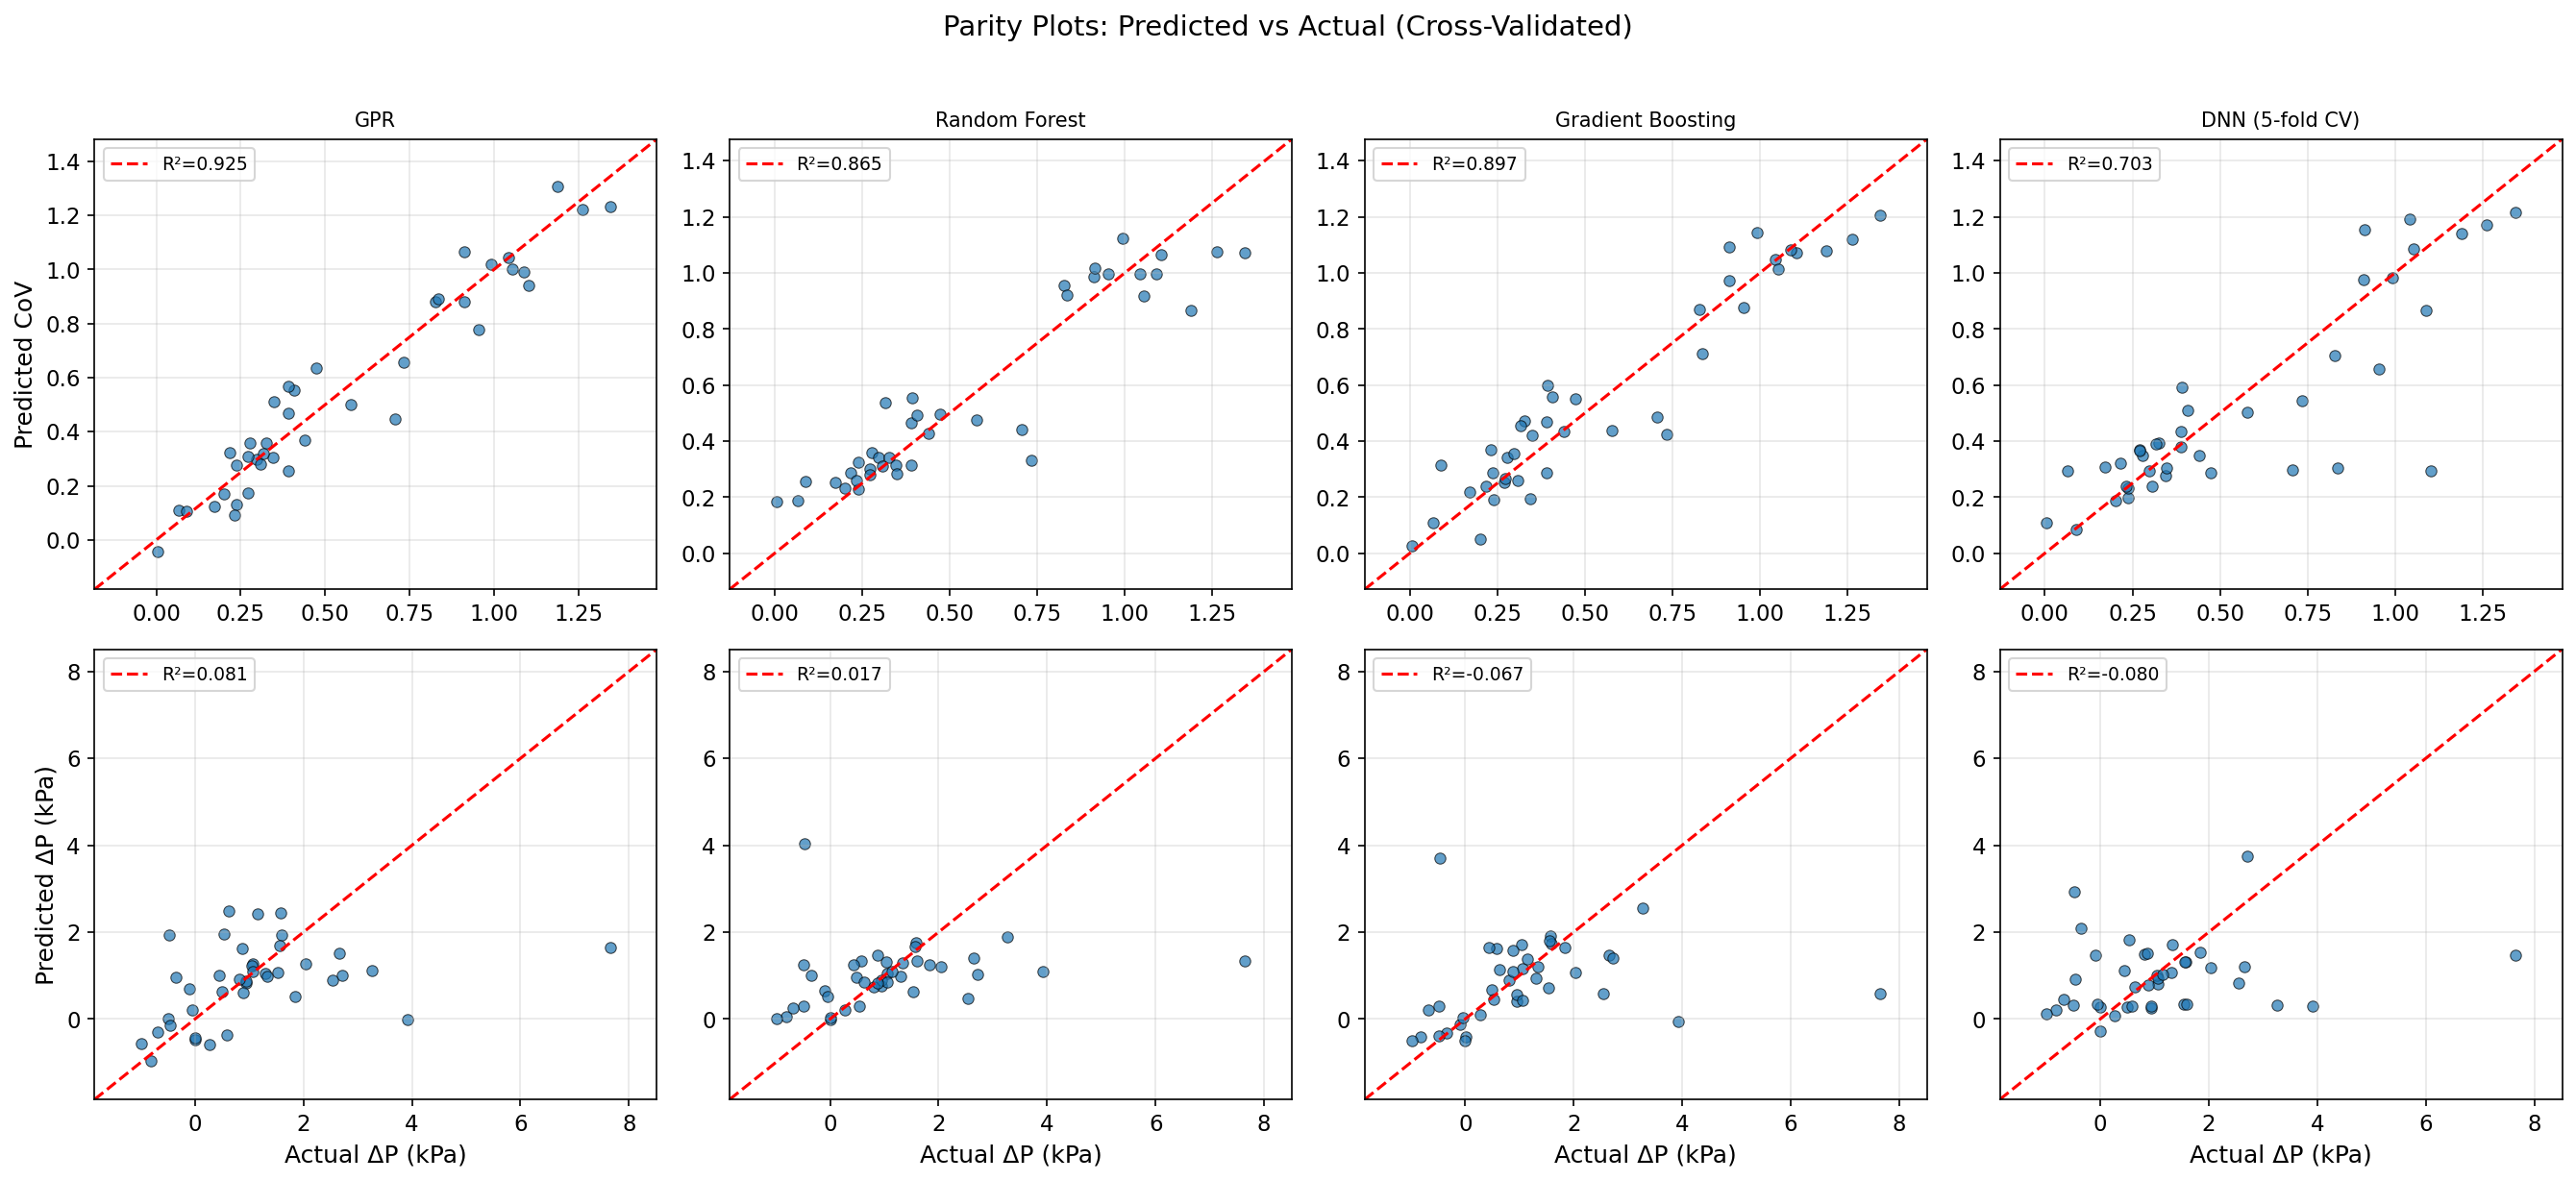
\includegraphics[width=\linewidth]{fig_parity_all_models.png}
                \caption{Parity plots (predicted vs actual).
                GPR has the tightest scatter for CoV.}
            \end{figure}
        \end{column}
    \end{columns}
\end{frame}

% ─── SLIDE 14: NSGA-II RESULTS ──────────────────────────────────────────
\begin{frame}{NSGA-II Optimisation: Pareto Fronts from GPR}
    \begin{columns}[T]
        \begin{column}{0.52\textwidth}
            \centering
            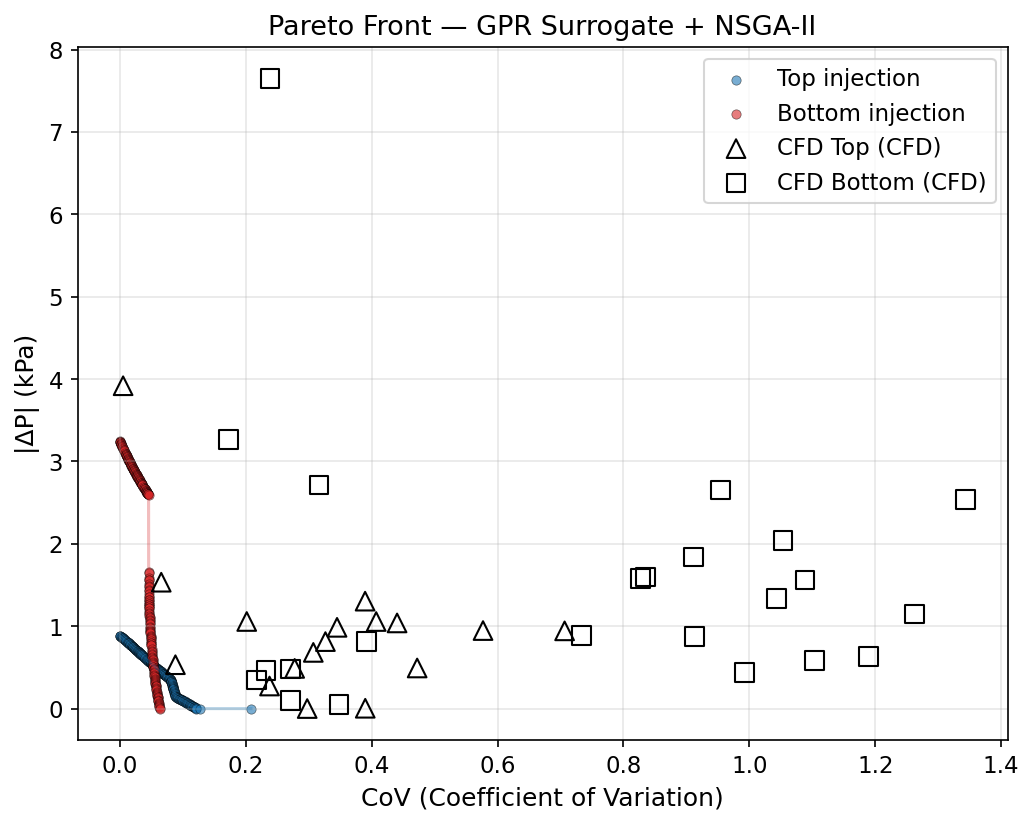
\includegraphics[width=0.95\linewidth]{fig_pareto_front_surrogate.png}\\[-0.3em]
            {\scriptsize NSGA-II Pareto fronts on GPR surrogate
            (200 pop, 150 gen).
            Hollow = CFD; solid = surrogate.}
        \end{column}
        \begin{column}{0.46\textwidth}
            \small
            \textbf{Knee-point designs} (closest to utopia):

            \vspace{0.3em}
            \begin{exampleblock}{\small Top Injection Knee}
                \scriptsize
                $\alpha = 30^\circ$, $d/D = 0.45$, VR $= 5.82$\\
                CoV $\approx 0.089$, $|\Delta P| \approx 0.14$~kPa
            \end{exampleblock}

            \vspace{0.1em}
            \begin{block}{\small Bottom Injection Knee}
                \scriptsize
                $\alpha = 90^\circ$, $d/D = 0.26$, VR $= 5.84$\\
                CoV $\approx 0.048$, $|\Delta P| \approx 0.97$~kPa
            \end{block}

            \vspace{0.3em}
            Both knee points maximise VR - consistent with SHAP:
            \textbf{injection side} and \textbf{VR} are the two
            dominant features.

            \vspace{0.2em}
            Top injection achieves a better trade-off: lower $|\Delta P|$
            for comparable CoV.
        \end{column}
    \end{columns}
\end{frame}

% ═══════════════════════════════════════════════════════════════════════════
\section{Summary}
% ═══════════════════════════════════════════════════════════════════════════

% ─── SLIDE 15: LIMITATIONS & FUTURE WORK ────────────────────────────────
\begin{frame}[fragile]{Limitations and Future Work}
    \begin{columns}[T]
        \begin{column}{0.48\textwidth}
            \textbf{Current limitations:}
            \begin{itemize}
                \item \textbf{$|\Delta P|$ surrogate unreliable} -
                      acoustic noise in compressible transient solver.
                \item \textbf{Two angles only} ($30^\circ$, $90^\circ$).
                \item \textbf{Single Reynolds number}
                      ($u_{\text{main}} = 10$~m/s).
                \item \textbf{$N = 40$ cases} - insufficient for the
                      DNN architecture ($\sim$17\,k parameters).
                \item Mesh convergence verified at one design point;
                      same baseline mesh used for all cases.
            \end{itemize}
        \end{column}
        \begin{column}{0.50\textwidth}
            \textbf{Planned next steps:}

            \vspace{0.3em}
            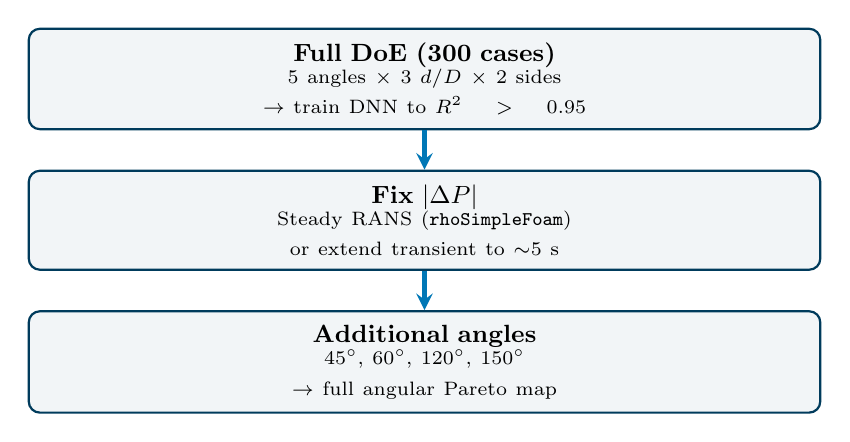
\begin{tikzpicture}[
                node distance=0.5cm,
                phasebox/.style={fill=iitdNavy!5, draw=iitdNavy, thick,
                                 rounded corners=4pt, text width=0.8\linewidth,
                                 align=center, font=\small, inner sep=5pt},
                arrow/.style={->, >=stealth, ultra thick, color=iitdAccent}
            ]
                \node[phasebox] (p1) {\textbf{Full DoE (300 cases)}\\
                    \scriptsize 5 angles $\times$ 3 $d/D$ $\times$ 2 sides\\
                    $\to$ train DNN to $R^2 > 0.95$};
                \node[phasebox, below=of p1] (p2) {\textbf{Fix $|\Delta P|$}\\
                    \scriptsize Steady RANS (\texttt{rhoSimpleFoam})\\
                    or extend transient to $\sim$5~s};
                \node[phasebox, below=of p2] (p3) {\textbf{Additional angles}\\
                    \scriptsize $45^\circ$, $60^\circ$, $120^\circ$, $150^\circ$\\
                    $\to$ full angular Pareto map};
                \draw[arrow] (p1) -- (p2);
                \draw[arrow] (p2) -- (p3);
            \end{tikzpicture}
        \end{column}
    \end{columns}
\end{frame}

% ─── SLIDE 17: CONCLUSIONS ──────────────────────────────────────────────
\begin{frame}{Conclusions}
    \begin{enumerate}
        \item \textbf{First multi-objective CFD study} of H$_2$ T-junction injection
              with angle as a design variable.
              40 validated RANS cases across 4 campaigns.

        \vspace{0.3em}
        \item \textbf{$30^\circ$ top injection dominates all other configurations.}
              Median CoV reduction: $-46\%$; median $|\Delta P|$ reduction: $-63\%$
              vs $90^\circ$ (all 7 matched pairs).

        \vspace{0.3em}
        \item \textbf{Top injection is strictly superior to bottom.}
              All 17 matched pairs favour top ($p = 1.5 \times 10^{-5}$).
              Median CoV degradation from top $\to$ bottom: $+109\%$ ($90^\circ$),
              $+324\%$ ($30^\circ$).

        \vspace{0.3em}
        \item \textbf{Buoyancy is the key mechanism:} top injection spreads H$_2$
              laterally (large interfacial area); bottom lifts a coherent column.

        \vspace{0.3em}
        \item \textbf{GPR surrogate} achieves $R^2 = 0.93$ for CoV;
              NSGA-II Pareto search identifies optimal knee-point designs
              in seconds.

        \vspace{0.3em}
        \item \textbf{All code, data and figures} are open-source at
              \url{https://github.com/Yash04dsr/MTP-Work}.
    \end{enumerate}
\end{frame}

% ─── SLIDE 18: CASE STRUCTURE & CODE ───────────────────────────────────
\begin{frame}[fragile]{OpenFOAM Case Structure \& Code Availability}
    \begin{columns}[T]
        \begin{column}{0.48\textwidth}
            \textbf{Each DoE case directory:}

            \vspace{0.3em}
            \ttfamily\scriptsize
            \begin{tabular}{@{}l@{}}
                case\_XX/ \\
                \hspace{0.6em}$\vdash$\hspace{0.3em} 0/\hspace{3.5em}{\rmfamily\itshape Boundary conditions} \\
                \hspace{0.6em}$\mid$\hspace{0.6em} $\vdash$ U, p\_rgh, H2, CH4, \ldots \\
                \hspace{0.6em}$\vdash$\hspace{0.3em} constant/ \\
                \hspace{0.6em}$\mid$\hspace{0.6em} $\vdash$ polyMesh/\hspace{0.5em}{\rmfamily\itshape Mesh} \\
                \hspace{0.6em}$\mid$\hspace{0.6em} $\vdash$ thermophysicalProperties \\
                \hspace{0.6em}$\mid$\hspace{0.6em} $\vdash$ turbulenceProperties \\
                \hspace{0.6em}$\vdash$\hspace{0.3em} system/ \\
                \hspace{0.6em}$\mid$\hspace{0.6em} $\vdash$ controlDict, fvSchemes \\
                \hspace{0.6em}$\mid$\hspace{0.6em} $\vdash$ fvSolution \\
                \hspace{0.6em}$\mid$\hspace{0.6em} $\vdash$ snappyHexMeshDict \\
                \hspace{0.6em}$\vdash$\hspace{0.3em} generateSTL.py \\
                \hspace{0.6em}$\vdash$\hspace{0.3em} Allrun\hspace{1.5em}{\rmfamily\itshape Full pipeline script} \\
                \hspace{0.6em}$\vdash$\hspace{0.3em} case.env, case\_info.json \\
                \hspace{0.6em}$\vdash$\hspace{0.3em} figures/\hspace{1em}{\rmfamily\itshape 13 PNG per case} \\
                \hspace{0.6em}$\vdash$\hspace{0.3em} postProcessing/ \\
                \hspace{0.6em}$\vdash$\hspace{0.3em} log.solver \\
            \end{tabular}
            \rmfamily
        \end{column}
        \begin{column}{0.50\textwidth}
            \textbf{DoE automation scripts:}
            \begin{itemize}\small\setlength{\itemsep}{2pt}
                \item \texttt{lhs\_design.py} - LHS sampling
                \item \texttt{stamp\_cases.py} - case materialiser
                \item \texttt{run\_doe.sh} - resilient orchestrator
                \item \texttt{all\_metrics.py} - CoV, $|\Delta P|$
                \item \texttt{make\_figures.py} - visualisations
                \item \texttt{cross\_analysis.py} - campaign comparison
                \item \texttt{train\_surrogate.py} - GPR + NSGA-II
            \end{itemize}

            \vspace{0.5em}
            \textbf{All code, data, and figures:}

            \vspace{0.3em}
            \centering
            \url{https://github.com/Yash04dsr/MTP-Work}

            \vspace{0.5em}
            \flushleft
            {\small 40 cases $\times$ 13 figures = 520 visualisations,\\
            plus cross-campaign analysis and surrogate model.}
        \end{column}
    \end{columns}
\end{frame}

% ─── SLIDE 19: BOUNDARY CONDITIONS ─────────────────────────────────────
\begin{frame}{Boundary Conditions Summary}
    \small
    \begin{columns}[T]
        \begin{column}{0.48\textwidth}
            \textbf{Velocity (U):}
            \begin{table}
                \centering\scriptsize
                \begin{tabular}{@{}ll@{}}
                    \toprule
                    \textbf{Patch} & \textbf{BC} \\
                    \midrule
                    main\_inlet & $\tfrac{1}{7}$-power-law profile \\
                    branch\_inlet & $\tfrac{1}{7}$-power-law profile \\
                    outlet & pressureInletOutletVelocity \\
                    wall & noSlip \\
                    sym & symmetryPlane \\
                    \bottomrule
                \end{tabular}
            \end{table}

            \vspace{0.2em}
            \textbf{Species (H$_2$ / CH$_4$):}
            \begin{table}
                \centering\scriptsize
                \begin{tabular}{@{}lcc@{}}
                    \toprule
                    \textbf{Patch} & \textbf{H$_2$} & \textbf{CH$_4$} \\
                    \midrule
                    main\_inlet & 0 & 1 \\
                    branch\_inlet & 1 & 0 \\
                    outlet & inletOutlet & inletOutlet \\
                    wall & zeroGradient & zeroGradient \\
                    \bottomrule
                \end{tabular}
            \end{table}

            \vspace{0.2em}
            \textbf{Temperature:} fixed at 288~K everywhere\\
            (energy equation disabled - isothermal).
        \end{column}
        \begin{column}{0.50\textwidth}
            \textbf{Pressure ($p_{\mathrm{rgh}}$):}
            \begin{table}
                \centering\scriptsize
                \begin{tabular}{@{}ll@{}}
                    \toprule
                    \textbf{Patch} & \textbf{BC} \\
                    \midrule
                    main\_inlet & fixedFluxPressure \\
                    branch\_inlet & fixedFluxPressure \\
                    outlet & prghPressure (69~bar ref) \\
                    wall & fixedFluxPressure \\
                    \bottomrule
                \end{tabular}
            \end{table}

            \vspace{0.2em}
            \textbf{Turbulence ($k$, $\omega$):}
            \begin{table}
                \centering\scriptsize
                \begin{tabular}{@{}lll@{}}
                    \toprule
                    \textbf{Patch} & $k$ & $\omega$ \\
                    \midrule
                    Inlets & TI = 5\% & $L_{\mathrm{mix}} = 0.07D$ \\
                    outlet & inletOutlet & inletOutlet \\
                    wall & kqRWallFn & omegaWallFn \\
                    \bottomrule
                \end{tabular}
            \end{table}

            \vspace{0.2em}
            \textbf{Per-case tokens} (stamped by \texttt{stamp\_cases.py}):\\[2pt]
            {\scriptsize
            \texttt{@UMAIN@}, \texttt{@UBRANCH@}, \texttt{@D1@},
            \texttt{@D2@}, \texttt{@ZJCT@}, \texttt{@K\_MAIN@},
            \texttt{@K\_BRANCH@}, \texttt{@OMEGA\_MAIN@},
            \texttt{@OMEGA\_BRANCH@}}
        \end{column}
    \end{columns}
\end{frame}

% ─── SLIDE 20: REFERENCES ──────────────────────────────────────────────
\begin{frame}{Key References}
    \small
    \begin{itemize}\setlength{\itemsep}{0.6em}
        \item Y.~Tian, T.~Tian, G.~Ren, and J.~Zhang.
        ``Numerical Simulation of Hydrogen Mixing Process in T-Junction Natural Gas Pipeline.''
        \textit{Energies}, vol.~16, no.~1, 2023.

        \item Y.~Su, J.~Li, W.~Guo, Y.~Zhao, et al.
        ``Prediction of Mixing Uniformity of Hydrogen Injection in Natural Gas Pipeline Based on a Deep Learning Model.''
        \textit{Energies}, vol.~15, no.~22, 2022.

        \item A.~K.~Arya, R.~Katiyar, P.~Senthil~Kumar, et al.
        ``A multi-objective model for optimizing hydrogen injected-high pressure natural gas pipeline networks.''
        \textit{Int. Journal of Hydrogen Energy}, vol.~48, 2023.

        \item N.~A.~N.~M.~N.~Azman et al.
        ``Hydrogen-Natural Gas Co-Blending: Performance Analysis with CFD and Static Mixers.''
        \textit{Chemical Engineering Transactions}, vol.~122, 2025.
    \end{itemize}
\end{frame}

% ─── SLIDE 21: THANK YOU ────────────────────────────────────────────────
\begin{frame}[plain]
    
\begin{tikzpicture}[remember picture, overlay]
        \fill[left color=iitdDark, right color=iitdAccent!80!iitdNavy]
            (current page.south west) rectangle (current page.north east);
        \fill[white, opacity=0.06]
            ([xshift=-2cm, yshift=-3cm]current page.north east) circle (7cm);
        \fill[white, opacity=0.04]
            ([xshift=3cm, yshift=2cm]current page.south west) circle (5cm);
    \end{tikzpicture}
    \vfill
    \begin{center}
        {\fontsize{28}{34}\selectfont\bfseries\color{white}Thank You}\\[16pt]
        {\Large\color{white}Questions?}\\[20pt]
        {\color{white!70}\rule{5cm}{0.5pt}}\\[20pt]
        {\large\color{white}\textbf{Sakhare Yash Balram}}\\[8pt]
        {\normalsize\color{white!90}%
         Department of Chemical Engineering\\
         Indian Institute of Technology Delhi}\\[12pt]
        {\normalsize\color{white!80}%
         \texttt{ch7221496@iitd.ac.in}}\\[8pt]
        {\small\color{white!60}%
         \url{https://github.com/Yash04dsr/MTP-Work}}
    \end{center}
    \vfill
\end{frame}

\end{document}
